\documentclass[11pt,a4paper]{article}
\usepackage{fontspec}
\setmainfont[Path=fonts/,BoldFont=NotoSerif-Bold.ttf,ItalicFont=NotoSerif-Italic.ttf,BoldItalicFont=NotoSerif-BoldItalic.ttf]{NotoSerif-Regular.ttf}
\setsansfont[Path=fonts/,BoldFont=NotoSans-Bold.ttf,ItalicFont=NotoSans-Italic.ttf,BoldItalicFont=NotoSans-BoldItalic.ttf]{NotoSans-Regular.ttf}
\usepackage[a4paper,margin=20mm]{geometry}
\usepackage{amsmath,amssymb,booktabs,array,longtable,pdflscape,graphicx,caption,hyperref}
\hypersetup{hidelinks}
\captionsetup{font=small,labelfont=bf}
\renewcommand{\thetable}{S\arabic{table}}
\renewcommand{\thefigure}{S\arabic{figure}}
\newcounter{supptablepanel}
\renewcommand{\theHtable}{\arabic{table}.\arabic{supptablepanel}}
\renewcommand{\thesubsection}{S\arabic{subsection}}
\renewcommand{\thesubsubsection}{\thesubsection.\arabic{subsubsection}}
\setlength{\parindent}{0pt}
\setlength{\parskip}{5pt}
\setlength{\LTpre}{8pt}
\setlength{\LTpost}{8pt}
\newcolumntype{L}[1]{>{\raggedright\arraybackslash}p{#1}}
\setlength{\emergencystretch}{2em}
\begin{document}
\special{pdf:minorversion 7}
\begin{center}\Large\textbf{Supplementary Material}\end{center}
\subsection{Dataset, Labeling, and Data Integrity}\label{sec:supp_1}
The analysis included 20 recording sessions from 10 participants, as reported in the main manuscript. Recording duration totaled 17.40 h: 11.33 h Awake and 6.07 h Drowsy. Labels were assigned using the Karolinska Sleepiness Scale (KSS), with video observation used for cross-checking. Participant--session linkage was unavailable. Primary inference therefore used recording sessions and does not establish participant-level effects.

The data contained 1,620,038 samples. Recording session 01 was sampled at 50 Hz and the remaining sessions at approximately 25 Hz. Sampling rates were estimated from the reciprocal of the median positive timestamp interval. Integrity checks found strictly increasing timestamps, no duplicates or invalid labels, and no missing, non-numeric, or infinite signal/time values. Raw PPG, processed PPG, and labels shared the same row axis. All sessions passed integrity and analysis-eligibility checks (Table~\ref{tab:supp_dataset}).

There were 69 temporal gaps exceeding 1.5 times the median sampling interval; 62 exceeded twice this interval, and none exceeded five times it. Gaps remained discontinuities without interpolation. The labels contained 86 state transitions, none across a gap. Splitting at state changes and gaps yielded 175 contiguous state segments (93 Awake, 82 Drowsy), with median duration 260.04 s; 60 were shorter than 60 s, 78 shorter than 180 s, and 94 shorter than 300 s.

\begingroup\small
\setlength{\tabcolsep}{3pt}
\renewcommand{\arraystretch}{1.18}
\stepcounter{supptablepanel}
\begin{longtable}{L{\dimexpr0.12048\linewidth-1.68675\tabcolsep\relax}L{\dimexpr0.16867\linewidth-2.36145\tabcolsep\relax}L{\dimexpr0.15663\linewidth-2.19277\tabcolsep\relax}L{\dimexpr0.25301\linewidth-3.54217\tabcolsep\relax}L{\dimexpr0.08434\linewidth-1.18072\tabcolsep\relax}L{\dimexpr0.09639\linewidth-1.34940\tabcolsep\relax}L{\dimexpr0.12048\linewidth-1.68675\tabcolsep\relax}}
\caption{Dataset and integrity summary.}\label{tab:supp_dataset}\\
\toprule
Session & Samples & Estimated fs (Hz) & Awake /\allowbreak  Drowsy samples & Gaps & Integrity & Analysis eligible\\
\midrule\endfirsthead
\multicolumn{7}{l}{Table~\ref{tab:supp_dataset} (continued)}\\
\toprule
Session & Samples & Estimated fs (Hz) & Awake /\allowbreak  Drowsy samples & Gaps & Integrity & Analysis eligible\\
\midrule\endhead
\bottomrule\endfoot
\bottomrule\endlastfoot
01 & 117,828 & 50.000 & 77,805 /\allowbreak  40,023 & 0 & Pass & Yes\\
04 & 75,416 & 24.992 & 46,897 /\allowbreak  28,519 & 3 & Pass & Yes\\
05 & 91,211 & 25.003 & 59,235 /\allowbreak  31,976 & 4 & Pass & Yes\\
06 & 79,179 & 24.993 & 51,240 /\allowbreak  27,939 & 5 & Pass & Yes\\
07 & 79,768 & 24.994 & 59,225 /\allowbreak  20,543 & 3 & Pass & Yes\\
08 & 77,595 & 24.994 & 61,405 /\allowbreak  16,190 & 4 & Pass & Yes\\
09 & 119,272 & 25.001 & 83,631 /\allowbreak  35,641 & 8 & Pass & Yes\\
10 & 60,386 & 24.998 & 45,365 /\allowbreak  15,021 & 3 & Pass & Yes\\
11 & 61,582 & 24.994 & 33,062 /\allowbreak  28,520 & 2 & Pass & Yes\\
12 & 89,853 & 24.989 & 34,376 /\allowbreak  55,477 & 2 & Pass & Yes\\
13 & 76,473 & 25.000 & 40,272 /\allowbreak  36,201 & 2 & Pass & Yes\\
14 & 85,948 & 24.994 & 54,871 /\allowbreak  31,077 & 5 & Pass & Yes\\
15 & 69,362 & 24.996 & 54,511 /\allowbreak  14,851 & 6 & Pass & Yes\\
17 & 68,752 & 24.993 & 45,601 /\allowbreak  23,151 & 2 & Pass & Yes\\
18 & 69,937 & 24.997 & 30,634 /\allowbreak  39,303 & 3 & Pass & Yes\\
19 & 73,041 & 24.996 & 54,123 /\allowbreak  18,918 & 4 & Pass & Yes\\
21 & 69,660 & 25.000 & 41,549 /\allowbreak  28,111 & 2 & Pass & Yes\\
22 & 74,710 & 25.001 & 50,359 /\allowbreak  24,351 & 3 & Pass & Yes\\
23 & 109,452 & 24.997 & 87,703 /\allowbreak  21,749 & 3 & Pass & Yes\\
25 & 70,613 & 24.996 & 46,905 /\allowbreak  23,708 & 5 & Pass & Yes\\
Total & 1,620,038 & Mixed & 1,058,769 /\allowbreak  561,269 & 69 & 20/\allowbreak 20 & 20/\allowbreak 20\\
\end{longtable}
\endgroup
{\small State composition is a sample count, not a duration estimate. Gaps use the threshold of 1.5 times the median timestamp interval. Analysis eligibility does not imply that every sample entered a retained window.}\par
{\small State-duration support in the integrity summaries used sample-associated intervals, capping gaps at the median sampling interval and assigning one median interval to the final sample. Recording-duration totals in the text follow the main manuscript.}\par
\subsection{Preprocessing, Quality Control, and Retained-Window Counts}\label{sec:supp_2}
Raw PPG was multiplied by $-1$ and processed with a second-order Butterworth band-pass filter (0.5--8 Hz), applied forward and backward for zero phase. All subsequent QC and nonlinear analyses used processed PPG.

Artifact screening used complete, non-overlapping 5-s blocks of $\mathrm{round}(5f_s)$ samples within each recording session. Amplitude and roughness were defined as

\[\begin{gathered}A=Q_{0.95}(x)-Q_{0.05}(x),\\ R=\sqrt{\mathrm{mean}((\Delta x)^2)}.\end{gathered}\]
Here, $Q_p$ is the $p$th quantile and $\Delta x$ is the first difference. Each feature $F\in\{A,R\}$ was standardized across the complete blocks of the same session:

\[\begin{gathered}z_F=0.6745\,\frac{F-\mathrm{median}(F)}{\max(\mathrm{MAD}(F),\epsilon)}.\end{gathered}\]
With $\mathrm{MAD}(F)=\mathrm{median}(|F-\mathrm{median}(F)|)$ and machine epsilon $\epsilon$, a block was flagged when $z_A>4.5$ or $z_R>4.5$. All its samples were marked, and any analysis window containing a marked sample was excluded. Trailing incomplete blocks were not screened.

Within each same-state run, complete non-overlapping 60-s windows used $\mathrm{round}(60f_s)$ samples. Incomplete tails were discarded and windows crossing state boundaries were not formed. Candidates containing a timestamp interval greater than $1.5/f_s$ were excluded, with subsequent positions anchored to the original state run. The same procedure was used at 120 and 180 s.

Windows passing artifact and gap screening were assessed for variance stability using complete, non-overlapping 10-s subwindows of $\mathrm{round}(10f_s)$ samples; at least two were required. With $v_k=\mathrm{Var}(x_k)$ calculated using $\mathrm{ddof}=0$, the index was

\[\begin{gathered}S=\frac{\mathrm{IQR}(v)}{\max(\mathrm{median}(v),\epsilon)},\\ \mathrm{IQR}(v)=Q_{0.75}(v)-Q_{0.25}(v).\end{gathered}\]
Acceptance required $S\leq0.5$. This screen supported local quasi-stationarity through variance stability, rather than establishing full stationarity. At 60 s, variance screening retained 596 Awake and 305 Drowsy windows from 623 and 328 passing artifact/gap screening. Final cohorts totaled 901, 405, and 238 windows at 60, 120, and 180 s (Table~\ref{tab:supp_qc}).

The 30-s cohort comprised two consecutive halves of each accepted 60-s parent window. These halves inherited parent QC and were not independently variance-screened, yielding 1,192 Awake and 610 Drowsy windows (1,802 total). LLE fit acceptance was applied separately (Section~\ref{sec:supp_7}); nominal retention was 872/901 (96.78\%). The complete metric-specific counts are in Table~\ref{tab:supp_qc} and the preprocessing/retention illustration in Fig.~\ref{fig:supp_qc}.

\begingroup\small
\setlength{\tabcolsep}{3pt}
\renewcommand{\arraystretch}{1.18}
\stepcounter{supptablepanel}
\begin{longtable}{L{\dimexpr0.10526\linewidth-1.47368\tabcolsep\relax}L{\dimexpr0.09474\linewidth-1.32632\tabcolsep\relax}L{\dimexpr0.11579\linewidth-1.62105\tabcolsep\relax}L{\dimexpr0.17895\linewidth-2.50526\tabcolsep\relax}L{\dimexpr0.10526\linewidth-1.47368\tabcolsep\relax}L{\dimexpr0.20000\linewidth-2.80000\tabcolsep\relax}L{\dimexpr0.20000\linewidth-2.80000\tabcolsep\relax}}
\caption{QC stages and metric-specific retained-window counts.}\label{tab:supp_qc}\\
\toprule
Duration (s) & State & Post-SQI/\allowbreak gap & Variance-pass /\allowbreak  final non-LLE & LLE-valid & Variance-pass fraction & LLE-pass fraction\\
\midrule\endfirsthead
\multicolumn{7}{l}{Table~\ref{tab:supp_qc} (continued)}\\
\toprule
Duration (s) & State & Post-SQI/\allowbreak gap & Variance-pass /\allowbreak  final non-LLE & LLE-valid & Variance-pass fraction & LLE-pass fraction\\
\midrule\endhead
\bottomrule\endfoot
\bottomrule\endlastfoot
30 & Awake & Not applicable & 1,192 & 1,089 & Not applicable & 1089/\allowbreak 1192 (91.36\%)\\
30 & Drowsy & Not applicable & 610 & 549 & Not applicable & 549/\allowbreak 610 (90.00\%)\\
60 & Awake & 623 & 596 & 579 & 596/\allowbreak 623 (95.67\%) & 579/\allowbreak 596 (97.15\%)\\
60 & Drowsy & 328 & 305 & 293 & 305/\allowbreak 328 (92.99\%) & 293/\allowbreak 305 (96.07\%)\\
120 & Awake & 284 & 269 & 264 & 269/\allowbreak 284 (94.72\%) & 264/\allowbreak 269 (98.14\%)\\
120 & Drowsy & 148 & 136 & 135 & 136/\allowbreak 148 (91.89\%) & 135/\allowbreak 136 (99.26\%)\\
180 & Awake & 168 & 161 & 160 & 161/\allowbreak 168 (95.83\%) & 160/\allowbreak 161 (99.38\%)\\
180 & Drowsy & 86 & 77 & 77 & 77/\allowbreak 86 (89.53\%) & 77/\allowbreak 77 (100.00\%)\\
\end{longtable}
\endgroup
{\small Variance-pass fractions divide the final non-LLE count by the post-SQI/gap count. LLE-pass fractions divide accepted fits by the final non-LLE count. SQI denotes amplitude/roughness signal-quality screening.}\par
{\small At 30 s, post-SQI/gap and independent variance-pass stages are not applicable because parent QC is inherited. Cohorts at different durations share source recordings.}\par
\begin{figure}[p]
\centering
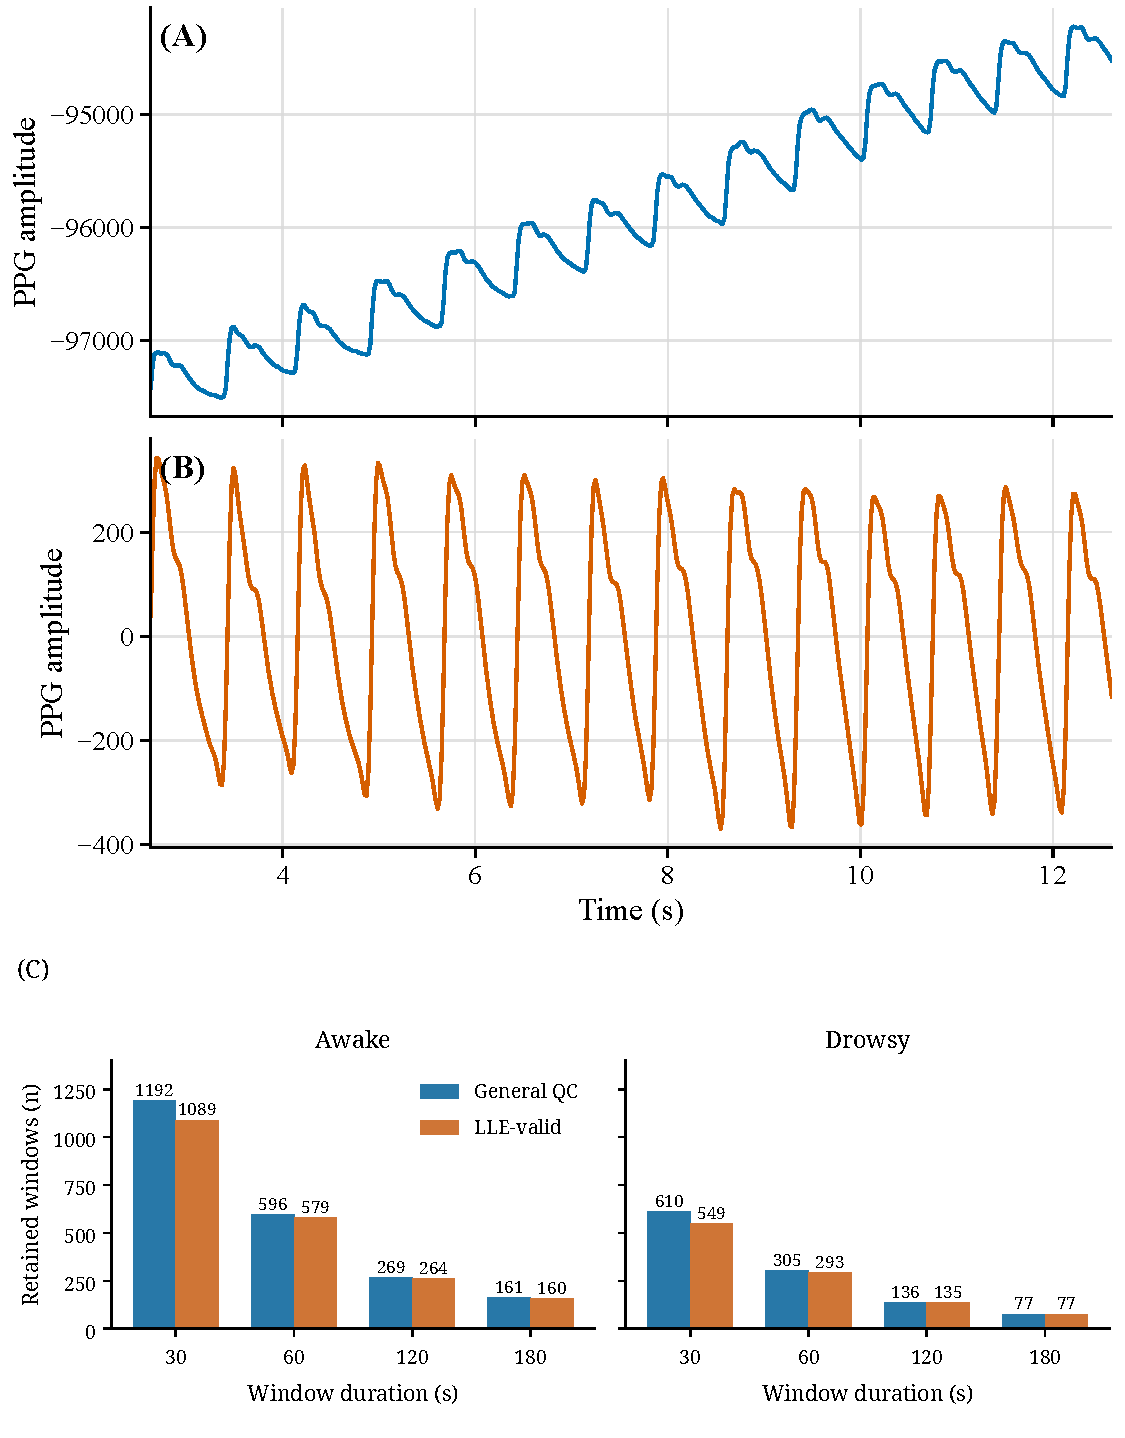
\includegraphics[width=\linewidth,height=.75\textheight,keepaspectratio]{figures/figure_S01.pdf}
\caption{Preprocessing and retained-window counts. (A) Sign-inverted raw PPG and (B) processed PPG after the 0.5--8 Hz zero-phase Butterworth filter. (C) General-QC and LLE-valid window counts by state and duration, as listed in Table~\ref{tab:supp_qc}. The 30-s windows are consecutive halves of accepted 60-s parents and inherit their QC.}\label{fig:supp_qc}
\end{figure}
\subsection{Frozen Nominal Analysis Configuration}\label{sec:supp_3}
The common nominal reconstruction and metric-specific settings are summarized in Table~\ref{tab:supp_nominal}A. The same embedding was used in both states. Windows were computational units and recording sessions were primary inferential units. Correction families are listed in Table~\ref{tab:supp_nominal}B; they are kept separate across analyses and configurations.

\begingroup\small
\setlength{\tabcolsep}{3pt}
\renewcommand{\arraystretch}{1.18}
\stepcounter{supptablepanel}
\begin{longtable}{L{\dimexpr0.17647\linewidth-0.70588\tabcolsep\relax}L{\dimexpr0.82353\linewidth-3.29412\tabcolsep\relax}}
\caption{Nominal configuration and statistical correction families.}\label{tab:supp_nominal}\\
\multicolumn{2}{l}{\textbf{Panel A. Nominal estimator configuration}}\\
\toprule
Component & Configuration\\
\midrule\endfirsthead
\multicolumn{2}{l}{Table~\ref{tab:supp_nominal} (continued)}\\
\toprule
Component & Configuration\\
\midrule\endhead
\bottomrule\endfoot
\bottomrule\endlastfoot
Input and windowing & Processed PPG; 60-s non-overlapping windows; 596 Awake + 305 Drowsy = 901.\\
Embedding & $\tau=0.16$ s; $m=8$; $\tau_{\mathrm{samples}}=\mathrm{round}(\tau f_s)$ (4/\allowbreak 8 samples at 25/\allowbreak 50 Hz).\\
Simplex Projection & $k=m+1=9$; Euclidean distance; normalized exponential weights; leave-one-out prediction; temporal exclusion $W=1.0$ s; 18 physical-time horizons from 0.04 to 4.00 s, converted using $\mathrm{round}(T_p f_s)$. Mean CC and Mean NRMSE are the means over horizons within each window.\\
RQA & Euclidean distance; per-window threshold targeting $\mathrm{RR}=0.02$; exclusion $W=(m-1)\tau_{\mathrm{samples}}$; $l_{\min}=v_{\min}=2$. Outputs: DET, $L_{\mathrm{mean}}$, LAM, TT. DET describes diagonal recurrence-line organization.\\
Rosenstein LLE & Nearest admissible Euclidean neighbor; spectral-mean-period temporal exclusion; maximum follow time 5 s; fit interval 0.80--1.30 s; $\geq$50 initial pairs; $\geq$30 pairs per fit point; $\geq$3 fit points; finite fit; $R^2\geq0.90$. Units: s$^{-1}$.\\
PPS & $M=39$ surrogates per tested window; tested noisy pseudoperiodic null; two-sided finite-sample rank test.\\
Aggregation and effects & Session-state medians of valid window metrics; paired $\Delta_i=\mathrm{Drowsy}_i-\mathrm{Awake}_i$; report the median paired difference. Simplex aggregation follows the within-window horizon means above.\\
Primary statistics & Two-sided Wilcoxon signed-rank test; matched-pairs rank-biserial correlation; 20,000 paired-session bootstrap resamples; percentile 95\% CI for the median paired difference; BH-FDR once across the seven nominal 60-s metrics.\\
\end{longtable}
\addtocounter{table}{-1}
\stepcounter{supptablepanel}
\begin{longtable}{L{\dimexpr0.17647\linewidth-0.70588\tabcolsep\relax}L{\dimexpr0.82353\linewidth-3.29412\tabcolsep\relax}}
\multicolumn{2}{l}{\textbf{Panel B. Statistical families}}\\
\toprule
Analysis family & Multiplicity reporting\\
\midrule\endfirsthead
\multicolumn{2}{l}{Table~\ref{tab:supp_nominal} (continued)}\\
\toprule
Analysis family & Multiplicity reporting\\
\midrule\endhead
\bottomrule\endfoot
\bottomrule\endlastfoot
Primary RQ2 & BH across 7 nominal 60-s metrics, once\\
Label sensitivity & BH across 4 headline metrics within each alternative rule\\
Delay/\allowbreak dimension sensitivity & BH across 4 headline metrics within each setting\\
RQA RR/\allowbreak Theiler sensitivity & Raw p only\\
LLE sensitivity & Raw p only\\
Window-length robustness & Raw p only\\
Repeated-session sensitivity & BH across 7 metrics per hypothetical matching\\
Symbolic dynamics & BH across 3 metrics per duration\\
PPS window-level rank tests & Unadjusted\\
PPS session-level gap family & BH across 12 tests: 6 metrics $\times$ 2 states\\
\end{longtable}
\endgroup
{\small The seven primary metrics are Mean CC, Mean NRMSE, DET, $L_{\mathrm{mean}}$, LAM, TT, and LLE. The four headline metrics are Mean CC, Mean NRMSE, DET, and LLE. Benjamini--Hochberg adjustment controls the false discovery rate within each specified family; families are not pooled across settings.}\par
{\small The PPS session-gap family contains the six non-LLE metrics in each state. Nominal reference rows in sensitivity tables retain the primary seven-metric family.}\par
\subsection{Phase-Space Reconstruction: AMI and FNN}\label{sec:supp_4}
Average Mutual Information (AMI) was calculated separately for each processed 60-s window using KSG estimator 1 with $k=3$, Chebyshev distance in joint space, and natural-log units (nats). Candidate delays ranged from one sample to $\mathrm{round}(f_s\times1.0~\mathrm{s})$ samples. Selection used the first strict interior local minimum without endpoint fallback; all 901 windows yielded a selected delay (Table~\ref{tab:supp_reconstruction_evidence}A).

Median selected delays were 0.160 s for Awake (Q25--Q75: 0.120--0.260 s) and 0.120 s for Drowsy (0.120--0.160 s). The median of 20 session medians supported the operational common delay $\tau=0.16$ s; 14/20 session medians were within $0.16\pm0.04$ s. This delay was shared across states and was not optimized for a state contrast.

False Nearest Neighbors (FNN) were evaluated over dimensions 1--10 using Euclidean nearest neighbors and Kennel-style criteria. A neighbor was false if additional-coordinate separation divided by the $m$-dimensional distance $R_m$ exceeded 15, or full $(m+1)$-dimensional distance divided by signal standard deviation exceeded 2. Self-matches and zero/near-zero distances were excluded; this diagnostic used no temporal exclusion.

At the nominal delay, median FNN across 20 session curves was 0.900\%, 0.886\%, and 1.008\% at $m=7,8,9$, respectively (Table~\ref{tab:supp_reconstruction_evidence}B). The common dimension $m=8$ was selected from this low-FNN region. At $m=8$, delays 0.12, 0.16, and 0.20 s yielded median FNN of 0.593\%, 0.886\%, and 1.284\%, with 19/20, 11/20, and 7/20 session curves below 1\% (Table~\ref{tab:supp_reconstruction_evidence}C). Neither parameter was treated as uniquely optimal, and the nominal setting did not require every session to have FNN below 1\%. These diagnostics describe operational reconstruction behavior (Fig.~\ref{fig:supp_reconstruction_evidence}); inferential sensitivity is addressed in Section~\ref{sec:supp_12_1}.

\begingroup\small
\setlength{\tabcolsep}{3pt}
\renewcommand{\arraystretch}{1.18}
\stepcounter{supptablepanel}
\begin{longtable}{L{\dimexpr0.14706\linewidth-1.76471\tabcolsep\relax}L{\dimexpr0.14706\linewidth-1.76471\tabcolsep\relax}L{\dimexpr0.14706\linewidth-1.76471\tabcolsep\relax}L{\dimexpr0.14706\linewidth-1.76471\tabcolsep\relax}L{\dimexpr0.14706\linewidth-1.76471\tabcolsep\relax}L{\dimexpr0.26471\linewidth-3.17647\tabcolsep\relax}}
\caption{AMI and FNN evidence for the common reconstruction.}\label{tab:supp_reconstruction_evidence}\\
\multicolumn{6}{l}{\textbf{Panel A. AMI-selected delays}}\\
\toprule
State & Windows & Median $\tau$ (s) & Q25 (s) & Q75 (s) & Successful selections\\
\midrule\endfirsthead
\multicolumn{6}{l}{Table~\ref{tab:supp_reconstruction_evidence} (continued)}\\
\toprule
State & Windows & Median $\tau$ (s) & Q25 (s) & Q75 (s) & Successful selections\\
\midrule\endhead
\bottomrule\endfoot
\bottomrule\endlastfoot
Awake & 596 & 0.160 & 0.120 & 0.260 & 596/\allowbreak 596\\
Drowsy & 305 & 0.120 & 0.120 & 0.160 & 305/\allowbreak 305\\
\end{longtable}
\addtocounter{table}{-1}
\stepcounter{supptablepanel}
\begin{longtable}{L{\dimexpr0.27273\linewidth-2.18182\tabcolsep\relax}L{\dimexpr0.27273\linewidth-2.18182\tabcolsep\relax}L{\dimexpr0.22727\linewidth-1.81818\tabcolsep\relax}L{\dimexpr0.22727\linewidth-1.81818\tabcolsep\relax}}
\multicolumn{4}{l}{\textbf{Panel B. FNN by dimension at $\tau$ = 0.16 s}}\\
\toprule
Dimension & Median FNN (\%) & Q25 (\%) & Q75 (\%)\\
\midrule\endfirsthead
\multicolumn{4}{l}{Table~\ref{tab:supp_reconstruction_evidence} (continued)}\\
\toprule
Dimension & Median FNN (\%) & Q25 (\%) & Q75 (\%)\\
\midrule\endhead
\bottomrule\endfoot
\bottomrule\endlastfoot
7 & 0.900 & 0.679 & 1.155\\
8 & 0.886 & 0.613 & 1.132\\
9 & 1.008 & 0.666 & 1.298\\
\end{longtable}
\addtocounter{table}{-1}
\stepcounter{supptablepanel}
\begin{longtable}{L{\dimexpr0.24390\linewidth-1.46341\tabcolsep\relax}L{\dimexpr0.34146\linewidth-2.04878\tabcolsep\relax}L{\dimexpr0.41463\linewidth-2.48780\tabcolsep\relax}}
\multicolumn{3}{l}{\textbf{Panel C. Delay sensitivity at m = 8}}\\
\toprule
$\tau$ (s) & Median FNN (\%) & Session curves <1\%\\
\midrule\endfirsthead
\multicolumn{3}{l}{Table~\ref{tab:supp_reconstruction_evidence} (continued)}\\
\toprule
$\tau$ (s) & Median FNN (\%) & Session curves <1\%\\
\midrule\endhead
\bottomrule\endfoot
\bottomrule\endlastfoot
0.12 & 0.593 & 19/\allowbreak 20\\
0.16 & 0.886 & 11/\allowbreak 20\\
0.20 & 1.284 & 7/\allowbreak 20\\
\end{longtable}
\endgroup
{\small Panel A summarizes selected delays across windows within each state; successful selections are relative to eligible windows. Panels B/C summarize session curves formed by median FNN across windows at each dimension. Their medians/quartiles and below-threshold counts are across 20 recording sessions. FNN is reported as a percentage.}\par
\begin{landscape}
\begin{figure}[p]
\centering
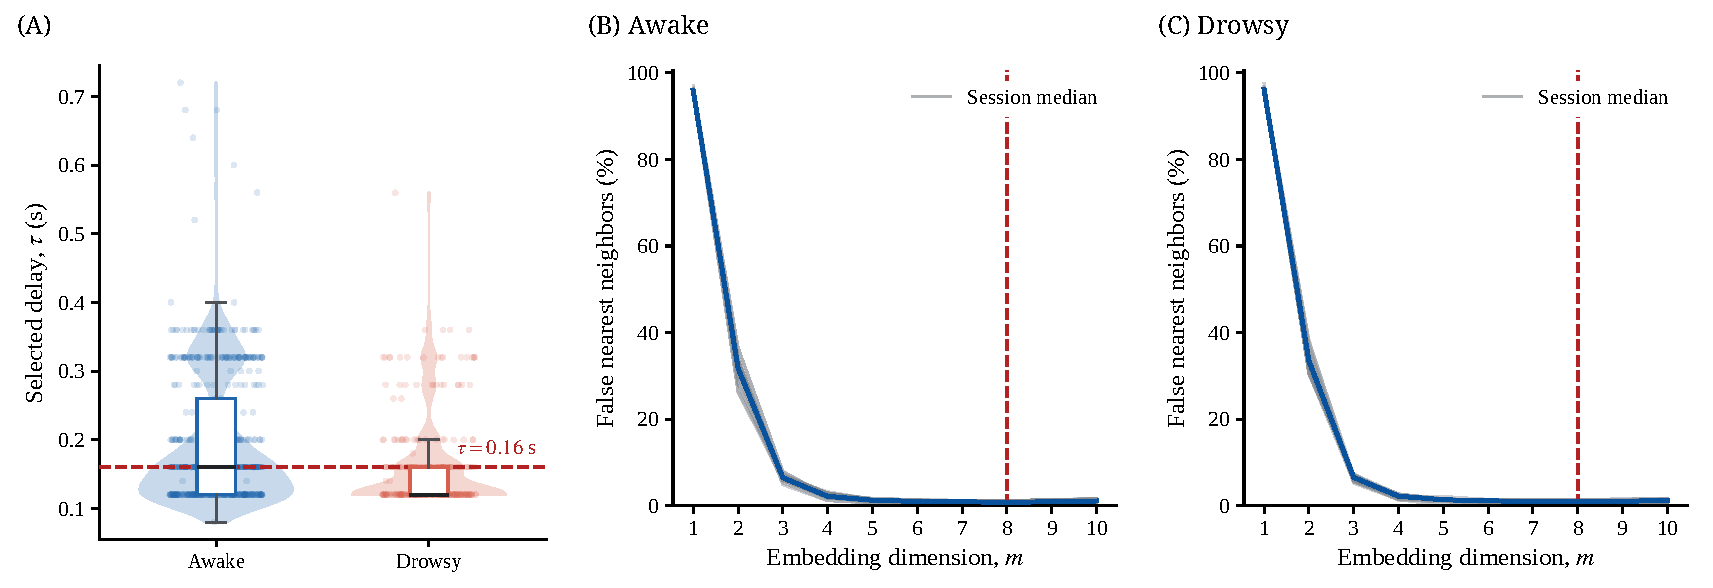
\includegraphics[width=\linewidth,height=.75\textheight,keepaspectratio]{figures/figure_S02.pdf}
\caption{Reconstruction evidence from processed 60-s PPG. (A) AMI-selected delays, with the common $\tau=0.16$ s. (B) Awake and (C) Drowsy FNN curves, with $m=8$ in a low-FNN region. The same reconstruction was used for both states. These diagnostics support an operational choice rather than a universal optimum.}\label{fig:supp_reconstruction_evidence}
\end{figure}
\end{landscape}
\subsection{Simplex Projection}\label{sec:supp_5}
Finite-horizon forecastability was assessed in the 901 retained windows. Each waveform was normalized as $u=(x-\bar{x})/\sigma_x$, using the whole-window population standard deviation ($\mathrm{ddof}=0$). The common reconstruction used $m=8$, $\tau=0.16$ s, and $d=\mathrm{round}(\tau f_s)$ samples.

Forward delay vectors were $\mathbf{z}_i=[u_i,u_{i+d},\ldots,u_{i+(m-1)d}]$, with final-coordinate index $t_i=i+(m-1)d$. At horizon $T_p$, offset $h=\mathrm{round}(T_pf_s)$ defined target $u_{t_i+h}$. Query and neighbor endpoints were restricted separately at each horizon so that vectors and targets remained within the same window. No cross-window prediction library was used.

Leave-one-out prediction used $k=m+1=9$ nearest admissible Euclidean neighbors. Self-matches were excluded, and $|t_j-t_i|>\mathrm{round}(f_sW)$ was required with $W=1.0$ s. For neighbor distances $D_j$ and smallest distance $D_1$, weights and predictions were

\[\begin{gathered}w_j=\frac{\exp(-D_j/D_1)}{\sum_{r=1}^{9}\exp(-D_r/D_1)},\\ \widehat{u}_{t_i+h}=\sum_{j=1}^{9}w_j u_{t_j+h}.\end{gathered}\]
If selected distances were no greater than machine epsilon, those neighbors shared the full weight equally and other selected neighbors received zero weight. Predictions required all nine admissible neighbors. For valid observed/predicted targets, CC and NRMSE were

\[\begin{gathered}\mathrm{CC}=\frac{\sum_i(y_i-\bar{y})(\widehat{y}_i-\bar{\widehat{y}})}{\sqrt{\sum_i(y_i-\bar{y})^2\sum_i(\widehat{y}_i-\bar{\widehat{y}})^2}},\\ \mathrm{NRMSE}=\frac{\sqrt{n^{-1}\sum_i(y_i-\widehat{y}_i)^2}}{\sigma_u}.\end{gathered}\]
Here, $n$ is the number of valid prediction pairs and $\sigma_u$ is the population standard deviation of the entire normalized window, equal to one up to numerical precision. It was not recomputed from a horizon-specific target subset. Higher CC and lower NRMSE indicate greater forecastability. Mean CC and Mean NRMSE were averaged across 18 horizons within each window, then summarized by the median of valid windows within each session and state, as reported in the manuscript. The 901 windows yielded 16,218 horizon-level outputs.

Table~\ref{tab:supp_simplex}A lists physical horizons and integer offsets at nominal sampling rates. Temporal-exclusion calibration tested $W\in\{0,0.2,0.4,0.6,0.8,1.0,1.5,2.0\}$ s. Adjacent-setting summaries pooled 120 session--state--duration combinations (20 sessions, two states, 60/120/180 s) and described absolute calibration changes, not state effects. The largest transition occurred from 0.6 to 0.8 s; 1.0 s was the first sustained stable setting after it (Table~\ref{tab:supp_simplex}B). Horizon behavior is illustrated in Fig.~\ref{fig:supp_simplex}.

\begingroup\small
\setlength{\tabcolsep}{3pt}
\renewcommand{\arraystretch}{1.18}
\stepcounter{supptablepanel}
\begin{longtable}{L{\dimexpr0.25000\linewidth-1.50000\tabcolsep\relax}L{\dimexpr0.37500\linewidth-2.25000\tabcolsep\relax}L{\dimexpr0.37500\linewidth-2.25000\tabcolsep\relax}}
\caption{Simplex horizons and temporal-exclusion calibration.}\label{tab:supp_simplex}\\
\multicolumn{3}{l}{\textbf{Panel A. Physical horizons and sample offsets}}\\
\toprule
Horizon (s) & 25-Hz offset (samples) & 50-Hz offset (samples)\\
\midrule\endfirsthead
\multicolumn{3}{l}{Table~\ref{tab:supp_simplex} (continued)}\\
\toprule
Horizon (s) & 25-Hz offset (samples) & 50-Hz offset (samples)\\
\midrule\endhead
\bottomrule\endfoot
\bottomrule\endlastfoot
0.04 & 1 & 2\\
0.08 & 2 & 4\\
0.12 & 3 & 6\\
0.16 & 4 & 8\\
0.20 & 5 & 10\\
0.28 & 7 & 14\\
0.40 & 10 & 20\\
0.60 & 15 & 30\\
0.80 & 20 & 40\\
1.00 & 25 & 50\\
1.20 & 30 & 60\\
1.60 & 40 & 80\\
2.00 & 50 & 100\\
2.40 & 60 & 120\\
2.80 & 70 & 140\\
3.20 & 80 & 160\\
3.60 & 90 & 180\\
4.00 & 100 & 200\\
\end{longtable}
\addtocounter{table}{-1}
\stepcounter{supptablepanel}
\begin{longtable}{L{\dimexpr0.16667\linewidth-1.66667\tabcolsep\relax}L{\dimexpr0.19444\linewidth-1.94444\tabcolsep\relax}L{\dimexpr0.19444\linewidth-1.94444\tabcolsep\relax}L{\dimexpr0.13889\linewidth-1.38889\tabcolsep\relax}L{\dimexpr0.30556\linewidth-3.05556\tabcolsep\relax}}
\multicolumn{5}{l}{\textbf{Panel B. Adjacent-setting calibration}}\\
\toprule
Adjacent W (s) & Median absolute ΔCC & Median absolute ΔNRMSE & Minimum support & Stability /\allowbreak  selection\\
\midrule\endfirsthead
\multicolumn{5}{l}{Table~\ref{tab:supp_simplex} (continued)}\\
\toprule
Adjacent W (s) & Median absolute ΔCC & Median absolute ΔNRMSE & Minimum support & Stability /\allowbreak  selection\\
\midrule\endhead
\bottomrule\endfoot
\bottomrule\endlastfoot
0.0 $\to$ 0.2 & 0.003550 & 0.003370 & 1.00 & Stable; before transition\\
0.2 $\to$ 0.4 & $2.204\times10^{-6}$ & $2.213\times10^{-6}$ & 1.00 & Stable; before transition\\
0.4 $\to$ 0.6 & 0.002137 & 0.002059 & 1.00 & Stable; before transition\\
0.6 $\to$ 0.8 & 0.020254 & 0.015614 & 1.00 & Largest transition; unstable\\
0.8 $\to$ 1.0 & 0.003605 & 0.003260 & 1.00 & Selected: W=1.0 s; sustained\\
1.0 $\to$ 1.5 & 0.008894 & 0.007937 & 1.00 & Stable; sustained\\
1.5 $\to$ 2.0 & 0.007034 & 0.006442 & 1.00 & Stable; sustained\\
\end{longtable}
\endgroup
{\small Panel A offsets illustrate 25/50 Hz; actual offsets use estimated session $f_s$. Panel B gives median absolute adjacent-setting changes over 120 combinations, with support defined as the minimum valid-prediction fraction.}\par
{\small Stability required both change rates, normalized to their respective largest rate, to be $\leq0.25$ and minimum support $\geq0.95$. Change rate is absolute change divided by the interval in $W$. Sustained stability required all subsequent pairs to pass; the selected upper setting was 1.0 s. These calibration quantities are not state-effect tests.}\par
\begin{figure}[p]
\centering
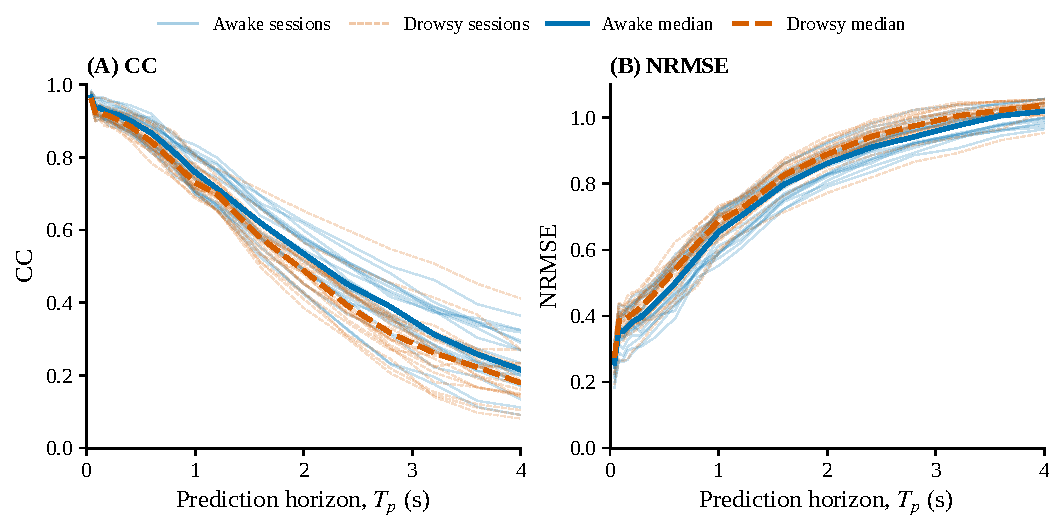
\includegraphics[width=\linewidth,height=.75\textheight,keepaspectratio]{figures/figure_S03.pdf}
\caption{Simplex horizon behavior in processed 60-s PPG. (A) CC and (B) NRMSE across 18 physical-time horizons from 0.04 to 4.00 s, using the common reconstruction and 1.0-s temporal exclusion. Session traces and state medians show finite-horizon forecastability; paired state effects are in Table~\ref{tab:supp_primary}.}\label{fig:supp_simplex}
\end{figure}
\subsection{Recurrence Quantification Analysis}\label{sec:supp_6}
RQA used Euclidean distances in the common reconstructed state space. A per-window threshold $\varepsilon$ targeted $\mathrm{RR}=0.02$, with recurrence defined by distance $\leq\varepsilon$. The line of identity and pairs with $|i-j|\leq W$ were excluded, where $W=(m-1)d$: 28 samples at approximately 25 Hz and 56 at 50 Hz (approximately 1.12 s). Density calibration counted eligible upper-triangle distances once. At a tied boundary, attainable counts below/at the boundary were compared with the target; the closer RR was selected, with lower RR on equal error. Equal distances were included or excluded together.

Let $C_{\mathrm{upper}}$ be eligible upper-triangle recurrent points and $P_d(l)$ count maximal diagonal runs of length $l$. With $l_{\min}=2$, diagonal recurrence-line organization and mean qualifying diagonal length were

\[\begin{gathered}\mathrm{DET}=\frac{\sum_{l\geq2}lP_d(l)}{C_{\mathrm{upper}}},\\ L_{\mathrm{mean}}=\frac{\sum_{l\geq2}lP_d(l)}{\sum_{l\geq2}P_d(l)}.\end{gathered}\]
Vertical runs were counted column-wise in the full symmetric recurrence matrix after the same mask. For recurrent-point count $C_{\mathrm{full}}$ and maximal vertical-run counts $P_v(v)$, with $v_{\min}=2$, laminarity and trapping time were

\[\begin{gathered}\mathrm{LAM}=\frac{\sum_{v\geq2}vP_v(v)}{C_{\mathrm{full}}},\\ \mathrm{TT}=\frac{\sum_{v\geq2}vP_v(v)}{\sum_{v\geq2}P_v(v)}.\end{gathered}\]
DET/LAM denominators included all recurrent points in their counting domains, including runs shorter than two. $L_{\mathrm{mean}}$ and TT averaged qualifying runs in sample-index line lengths, not seconds. The implementation returned zero when no qualifying runs were present, and zero fractions if the recurrence count was zero. DET describes diagonal recurrence-line organization; LAM/TT describe vertical organization, without a direct physical-determinism or autonomic interpretation. Fig.~\ref{fig:supp_rqa} illustrates recurrence geometry; nominal effects are in Table~\ref{tab:supp_primary} and estimator sensitivity in Section~\ref{sec:supp_12_2}.

\begin{figure}[p]
\centering
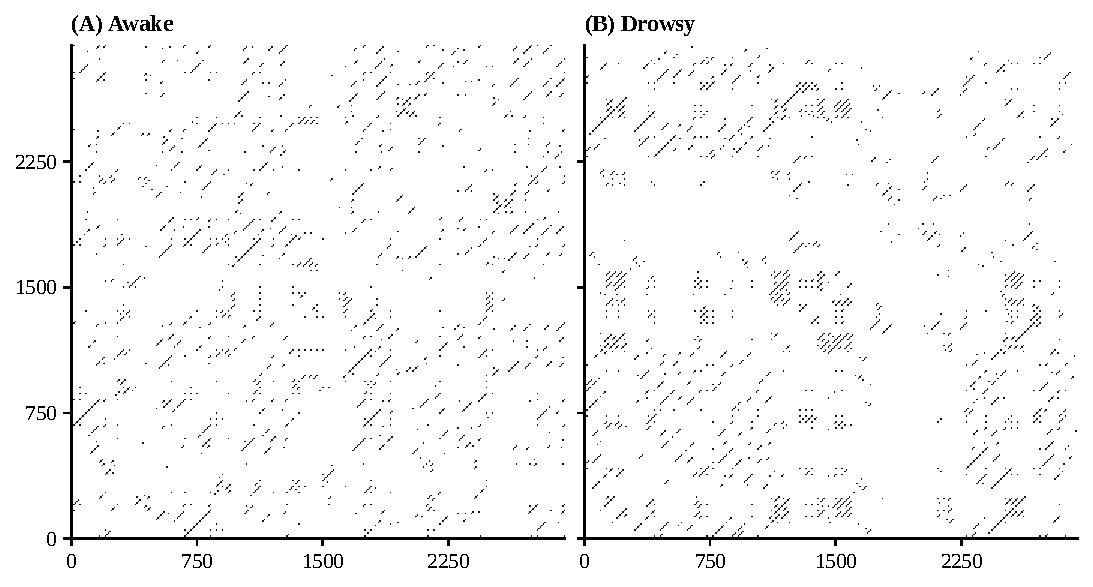
\includegraphics[width=\linewidth,height=.75\textheight,keepaspectratio]{figures/figure_S04.pdf}
\caption{Example Awake and Drowsy recurrence plots from recording session 01, using processed 60-s windows, the common embedding, $\mathrm{RR}=0.02$, and exclusion $W=(m-1)d$. Diagonal runs contribute to DET and $L_{\mathrm{mean}}$; vertical runs to LAM and TT. The plots illustrate recurrence geometry rather than inferential state effects.}\label{fig:supp_rqa}
\end{figure}
\subsection{Rosenstein Largest Lyapunov Exponent}\label{sec:supp_7}
The Rosenstein estimator assessed finite-window local trajectory divergence using the common embedding. Its temporal exclusion was based on the spectral mean period of the demeaned processed waveform. Power was squared Fourier magnitude in a one-sided spectrum, excluding DC and retaining positive frequencies through Nyquist without an additional frequency mask. For power $P_k$ at $f_k$,

\[\begin{gathered}\bar{f}=\frac{\sum_{k:f_k>0}f_kP_k}{\sum_{k:f_k>0}P_k},\\ T=\bar{f}^{-1},\\ W=\max\{1,\mathrm{round}(f_sT)\}.\end{gathered}\]
The first nearest Euclidean neighbor satisfying $|j-i|>W$ was selected. Distances $\leq\delta=10\epsilon_{\mathrm{machine}}\max\{\mathrm{std}(\mathbf{Z}),1\}\sqrt{m}$ were then rejected without replacing the neighbor; $\mathrm{std}(\mathbf{Z})$ is the population standard deviation across the state matrix. Admissible pairs were followed for at most 5 s. Pairs with in-window evolved endpoints and finite distance above $\delta$ contributed to the mean log-distance curve,

\[\begin{gathered}D(t)=\frac{1}{n_t}\sum_{j\in\mathcal{P}_t}\ln\|\mathbf{z}_{j+\ell}-\mathbf{z}_{\nu(j)+\ell}\|,\\ t=\ell/f_s.\end{gathered}\]
Here, $\nu(j)$ identifies the selected neighbor, $\mathcal{P}_t$ is the valid pair set at lag $\ell$, and $n_t$ is its size. Linear regression against time in seconds over inclusive 0.80--1.30 s gave the slope in s$^{-1}$ (Fig.~\ref{fig:supp_lle}). Acceptance required at least 50 initial pairs, 30 pairs per fit point, three finite fit points, a finite slope, and $R^2\geq0.90$.

Acceptance retained 872/901 input windows (96.78\%): 579 Awake and 293 Drowsy. Across all input windows, minimum initial pair count was 1,471, minimum pair count at a fit point was 1,366, and median fit $R^2$ was 0.973. Pair support therefore exceeded the operational minima throughout. The 29 rejected windows (17 Awake, 12 Drowsy) failed $R^2$, rather than pair-support criteria. These diagnostics include rejected fits; state comparisons use accepted fits only. LLE is a finite-data divergence estimate, not evidence establishing deterministic chaos. Nominal effects are in Table~\ref{tab:supp_primary}; perturbations are in Section~\ref{sec:supp_12_3}.

\begin{figure}[p]
\centering
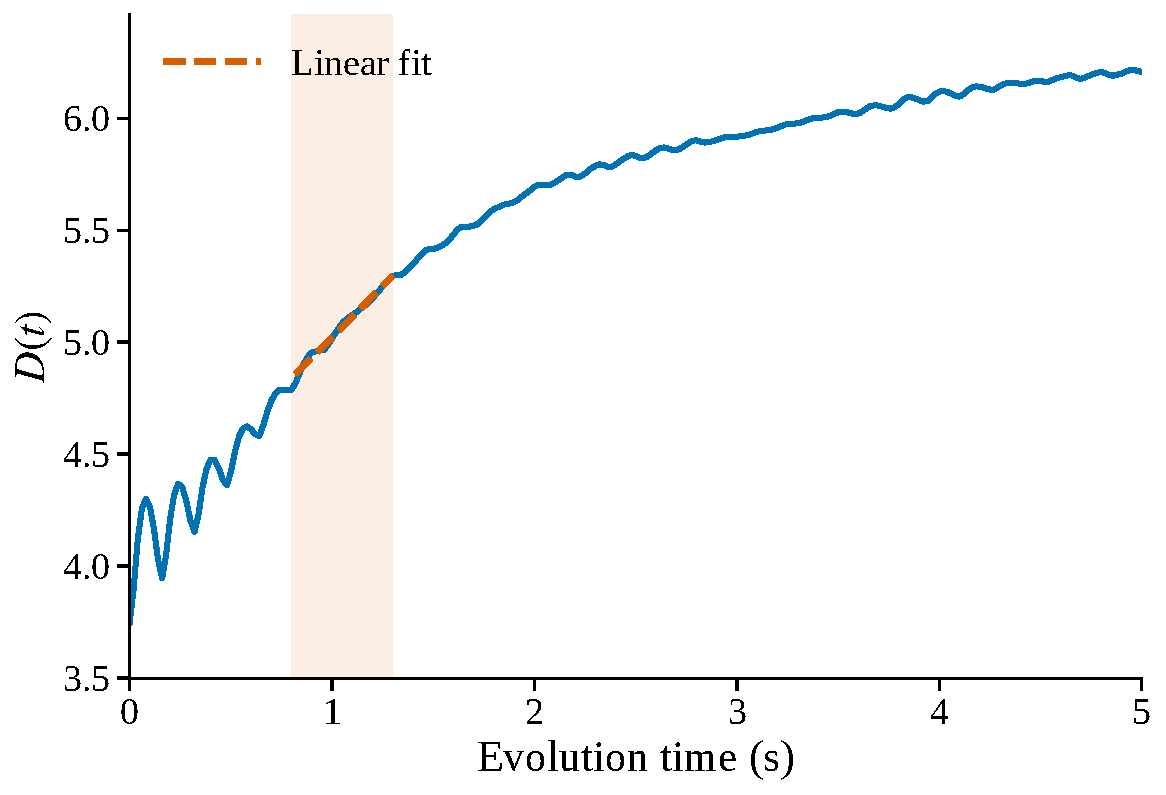
\includegraphics[width=\linewidth,height=.75\textheight,keepaspectratio]{figures/figure_S05.pdf}
\caption{Example Rosenstein mean log-distance curve $D(t)$ and linear fit from a processed 60-s Awake window in recording session 01. The fit spans 0.80--1.30 s. Acceptance criteria are defined in Section~\ref{sec:supp_7}. The slope is the finite-window LLE estimate in s$^{-1}$.}\label{fig:supp_lle}
\end{figure}
\subsection{Pseudoperiodic Surrogate Testing}\label{sec:supp_8}
Pseudoperiodic surrogates (PPS) tested a noisy pseudoperiodic null. Processed waveforms were forward-embedded using the common reconstruction and an initial index drawn uniformly from embedded states. For current state $\mathbf{s}$, candidate indices included all states with an observed successor, with probabilities

\[\begin{gathered}\Pr(j\mid\mathbf{s})=\frac{\exp[-(\|\mathbf{z}_j-\mathbf{s}\|-D_{\min})/\rho]}{\sum_{r=0}^{N_e-2}\exp[-(\|\mathbf{z}_r-\mathbf{s}\|-D_{\min})/\rho]},\end{gathered}\]
Here, $N_e$ is the number of embedded states and $D_{\min}$ the smallest candidate distance; subtracting it stabilizes the exponential without changing normalized probabilities. After selecting $j$, the surrogate continued at observed successor $j+1$. Self and temporally adjacent candidates were allowed; the last embedded state was excluded because it lacked a successor. The first coordinate of each visited state was emitted until the original window length was reached, without boundary wrapping.

Window-specific radius $\rho$ maximized the mean number of maximal consecutive source-index runs of length at least two, using three trials at each of 21 candidate radii; ties used the first maximum. Each window was compared with $M=39$ surrogates. The six non-LLE metrics shared an ensemble; LLE used a separate ensemble, retaining original-window exclusion but not imposing the original $R^2\geq0.90$ threshold on surrogate fits. LLE comparisons used the 579 Awake and 293 Drowsy original accepted fits.

For original value $a$ and surrogate values $s_1,\ldots,s_M$, the two-sided finite-sample test included ties in both tails:

\[\begin{gathered}p=\min\left\{1,\frac{2\min\left(1+\#\{s_b\leq a\},\;1+\#\{s_b\geq a\}\right)}{M+1}\right\}.\end{gathered}\]
The smallest attainable $p$ was $2/40=0.05$, with rejection at $p\leq0.05$ and no window-level adjustment. There were 24 exact original--surrogate ties across six-metric comparisons, none changing rejection at this threshold; included LLE comparisons had no ties.

Table~\ref{tab:supp_pps}A distinguishes pooled rejection percentages from median/IQR of 20 session-specific fractions. CC rejected in 374/596 Awake windows (62.75\% pooled; 60.66\% session median) and 229/305 Drowsy windows (75.08\%; 71.01\%). Expected original-minus-PPS directions were positive for CC, DET, $L_{\mathrm{mean}}$, and LLE and negative for NRMSE, LAM, and TT. One Drowsy LAM rejection had the opposite direction; all others followed the expected direction.

For session-gap inference (Table~\ref{tab:supp_pps}B), each window contributed its original value minus the median of 39 surrogates. Session-state median gaps were summarized and tested across 20 sessions, with BH correction over 12 metric--state tests. Rejection fractions are descriptive; no LLE gap CI, p, or q is included in this family.

PPS rejection indicates departure from the tested noisy pseudoperiodic null. It neither establishes deterministic chaos nor excludes all stochastic or structured pseudoperiodic models. Within-state rejection fractions are not a paired Awake--Drowsy test. An illustrative waveform and rejection heatmaps are shown in Fig.~\ref{fig:supp_pps}.

\begin{landscape}
\begingroup\small
\setlength{\tabcolsep}{3pt}
\renewcommand{\arraystretch}{1.18}
\stepcounter{supptablepanel}
\begin{longtable}{L{\dimexpr0.13592\linewidth-2.44660\tabcolsep\relax}L{\dimexpr0.09709\linewidth-1.74757\tabcolsep\relax}L{\dimexpr0.09709\linewidth-1.74757\tabcolsep\relax}L{\dimexpr0.09709\linewidth-1.74757\tabcolsep\relax}L{\dimexpr0.10680\linewidth-1.92233\tabcolsep\relax}L{\dimexpr0.12621\linewidth-2.27184\tabcolsep\relax}L{\dimexpr0.09709\linewidth-1.74757\tabcolsep\relax}L{\dimexpr0.12136\linewidth-2.18447\tabcolsep\relax}L{\dimexpr0.12136\linewidth-2.18447\tabcolsep\relax}}
\caption{PPS window rejection and session-level gap evidence.}\label{tab:supp_pps}\\
\multicolumn{9}{l}{\textbf{Panel A. Window-level rejection summaries}}\\
\toprule
Metric & State & Valid windows & Rejected n & Pooled (\%) & Session median (\%) & IQR (pp) & Expected-direction n & Opposite-direction n\\
\midrule\endfirsthead
\multicolumn{9}{l}{Table~\ref{tab:supp_pps} (continued)}\\
\toprule
Metric & State & Valid windows & Rejected n & Pooled (\%) & Session median (\%) & IQR (pp) & Expected-direction n & Opposite-direction n\\
\midrule\endhead
\bottomrule\endfoot
\bottomrule\endlastfoot
Mean CC & Awake & 596 & 374 & 62.75 & 60.66 & 16.98 & 374 & 0\\
Mean CC & Drowsy & 305 & 229 & 75.08 & 71.01 & 23.31 & 229 & 0\\
Mean NRMSE & Awake & 596 & 542 & 90.94 & 91.59 & 12.57 & 542 & 0\\
Mean NRMSE & Drowsy & 305 & 291 & 95.41 & 100.00 & 7.27 & 291 & 0\\
DET & Awake & 596 & 595 & 99.83 & 100.00 & 0.00 & 595 & 0\\
DET & Drowsy & 305 & 305 & 100.00 & 100.00 & 0.00 & 305 & 0\\
$L_{\mathrm{mean}}$ & Awake & 596 & 594 & 99.66 & 100.00 & 0.00 & 594 & 0\\
$L_{\mathrm{mean}}$ & Drowsy & 305 & 305 & 100.00 & 100.00 & 0.00 & 305 & 0\\
LAM & Awake & 596 & 537 & 90.10 & 95.50 & 16.36 & 537 & 0\\
LAM & Drowsy & 305 & 273 & 89.51 & 92.38 & 18.59 & 272 & 1\\
TT & Awake & 596 & 580 & 97.32 & 100.00 & 4.31 & 580 & 0\\
TT & Drowsy & 305 & 295 & 96.72 & 100.00 & 7.28 & 295 & 0\\
LLE & Awake & 579 & 545 & 94.13 & 96.30 & 7.28 & 545 & 0\\
LLE & Drowsy & 293 & 287 & 97.95 & 100.00 & 0.76 & 287 & 0\\
\end{longtable}
\clearpage
\addtocounter{table}{-1}
\stepcounter{supptablepanel}
\begin{longtable}{L{\dimexpr0.11200\linewidth-2.01600\tabcolsep\relax}L{\dimexpr0.08000\linewidth-1.44000\tabcolsep\relax}L{\dimexpr0.07200\linewidth-1.29600\tabcolsep\relax}L{\dimexpr0.10400\linewidth-1.87200\tabcolsep\relax}L{\dimexpr0.19200\linewidth-3.45600\tabcolsep\relax}L{\dimexpr0.11200\linewidth-2.01600\tabcolsep\relax}L{\dimexpr0.11200\linewidth-2.01600\tabcolsep\relax}L{\dimexpr0.08800\linewidth-1.58400\tabcolsep\relax}L{\dimexpr0.12800\linewidth-2.30400\tabcolsep\relax}}
\multicolumn{9}{l}{Table~\ref{tab:supp_pps} (continued)}\\
\multicolumn{9}{l}{\textbf{Panel B. Session-level original-minus-PPS gaps}}\\
\toprule
Metric & State & Sessions & Median gap & 95\% CI & Raw $p$ & $q_{\mathrm{BH}}$ & $r_{\mathrm{rb}}$ & Session median rejection (\%)\\
\midrule\endfirsthead
\multicolumn{9}{l}{Table~\ref{tab:supp_pps} (continued)}\\
\toprule
Metric & State & Sessions & Median gap & 95\% CI & Raw $p$ & $q_{\mathrm{BH}}$ & $r_{\mathrm{rb}}$ & Session median rejection (\%)\\
\midrule\endhead
\bottomrule\endfoot
\bottomrule\endlastfoot
Mean CC & Awake & 20 & +0.1192 & [0.1034, 0.1278] & $1.90735\times10^{-6}$ & $1.90735\times10^{-6}$ & +1.000 & 60.66\\
Mean CC & Drowsy & 20 & +0.1441 & [0.1245, 0.1906] & $1.90735\times10^{-6}$ & $1.90735\times10^{-6}$ & +1.000 & 71.01\\
Mean NRMSE & Awake & 20 & -0.1321 & [-0.1658, -0.1273] & $1.90735\times10^{-6}$ & $1.90735\times10^{-6}$ & -1.000 & 91.59\\
Mean NRMSE & Drowsy & 20 & -0.1557 & [-0.1901, -0.1370] & $1.90735\times10^{-6}$ & $1.90735\times10^{-6}$ & -1.000 & 100.00\\
DET & Awake & 20 & +0.1833 & [0.1727, 0.1939] & $1.90735\times10^{-6}$ & $1.90735\times10^{-6}$ & +1.000 & 100.00\\
DET & Drowsy & 20 & +0.1885 & [0.1713, 0.1971] & $1.90735\times10^{-6}$ & $1.90735\times10^{-6}$ & +1.000 & 100.00\\
$L_{\mathrm{mean}}$ & Awake & 20 & +1.1528 & [1.0947, 1.1891] & $1.90735\times10^{-6}$ & $1.90735\times10^{-6}$ & +1.000 & 100.00\\
$L_{\mathrm{mean}}$ & Drowsy & 20 & +1.1508 & [1.1023, 1.1815] & $1.90735\times10^{-6}$ & $1.90735\times10^{-6}$ & +1.000 & 100.00\\
LAM & Awake & 20 & -0.1244 & [-0.1411, -0.1130] & $1.90735\times10^{-6}$ & $1.90735\times10^{-6}$ & -1.000 & 95.50\\
LAM & Drowsy & 20 & -0.1266 & [-0.1282, -0.1091] & $1.90735\times10^{-6}$ & $1.90735\times10^{-6}$ & -1.000 & 92.38\\
TT & Awake & 20 & -0.1139 & [-0.1367, -0.0855] & $1.90735\times10^{-6}$ & $1.90735\times10^{-6}$ & -1.000 & 100.00\\
TT & Drowsy & 20 & -0.1188 & [-0.1283, -0.1077] & $1.90735\times10^{-6}$ & $1.90735\times10^{-6}$ & -1.000 & 100.00\\
\end{longtable}
\endgroup
{\small Panel A: CC/NRMSE are window-level horizon means. Pooled rejection equals rejected/valid windows $\times100$; session median and IQR summarize 20 session-specific fractions scaled by 100. Expected signs are for original minus PPS: positive for CC, DET, $L_{\mathrm{mean}}$, LLE and negative for NRMSE, LAM, TT. LLE uses 579/293 original accepted windows, versus 596/305 for other metrics.}\par
{\small Panel B: CI, Wilcoxon signed-rank p, $r_{\mathrm{rb}}$, and BH-adjusted q describe session-state median original-minus-PPS gaps across 20 sessions. BH covers the 12 six-metric--state tests once. Rejection fractions are descriptive and LLE has no gap inference in this family. Gap/CI units are samples for $L_{\mathrm{mean}}$/TT and dimensionless otherwise.}\par
\end{landscape}
\begin{figure}[p]
\centering
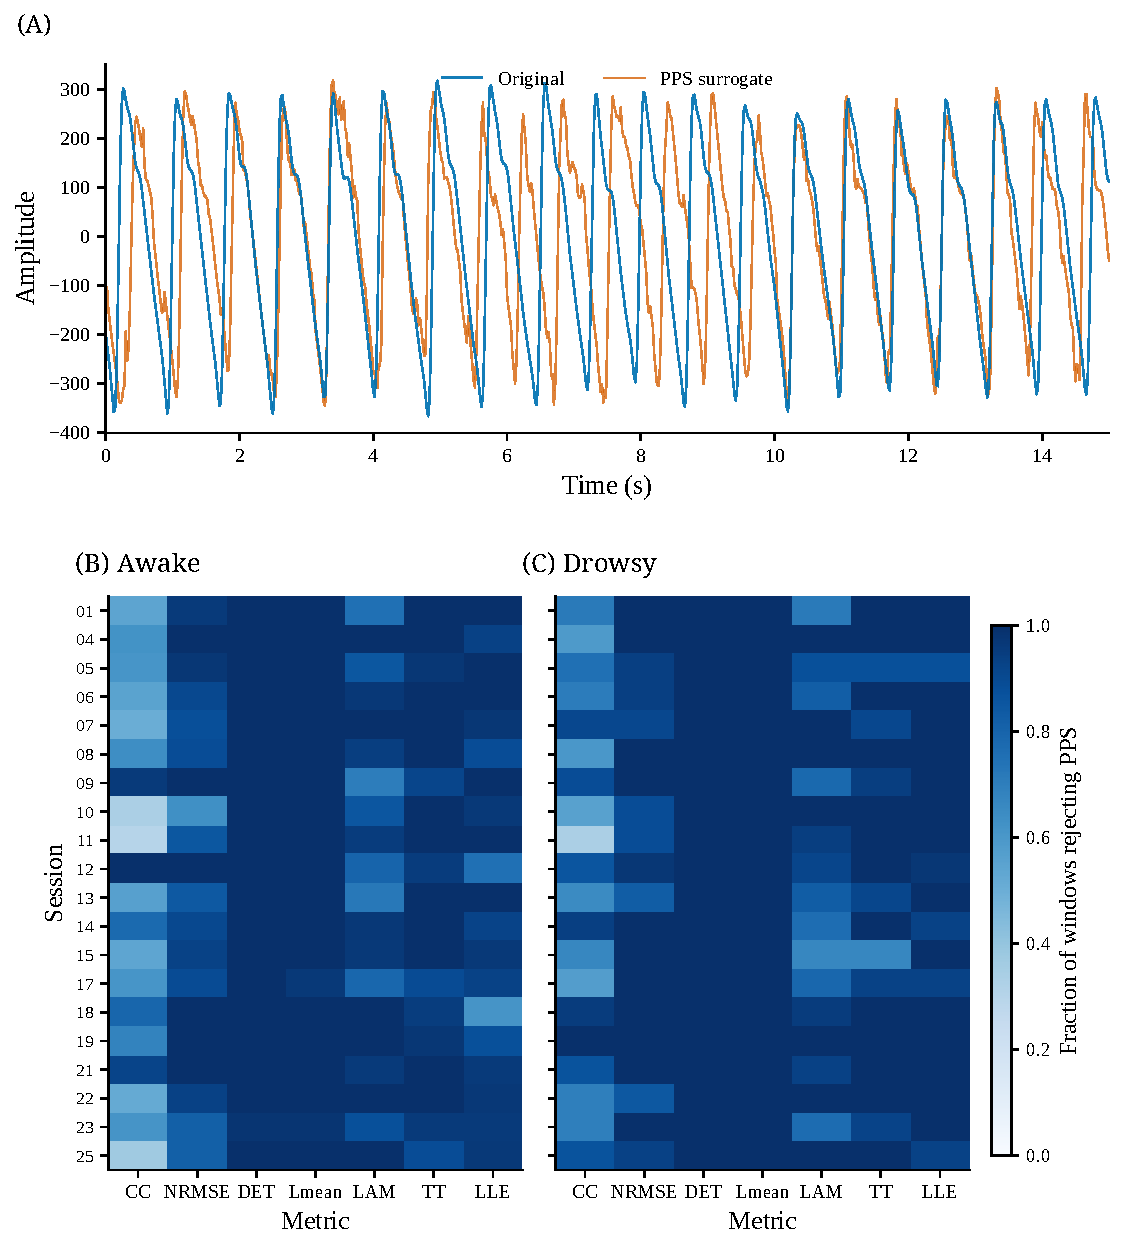
\includegraphics[width=\linewidth,height=.75\textheight,keepaspectratio]{figures/figure_S06.pdf}
\caption{PPS illustration and rejection patterns. (A) A 15-s view of original processed PPG and an illustrative surrogate from recording session 01. (B) Awake and (C) Drowsy session-specific fractions rejecting the tested noisy pseudoperiodic null. Tests use 39 surrogates, tie-inclusive two-sided ranks, and unadjusted $p\leq0.05$. LLE fractions use original accepted fits. The waveform is illustrative; heatmaps describe within-state rejection, not paired state effects.}\label{fig:supp_pps}
\end{figure}
\subsection{Statistical Framework and Multiplicity}\label{sec:supp_9}
Each metric was summarized by the median of valid windows within each recording session and state. For Simplex, window metrics were first averaged over horizons (Section~\ref{sec:supp_5}). Each of 20 sessions contributed a paired difference,

\[\begin{gathered}\Delta_i=\mathrm{Drowsy}_i-\mathrm{Awake}_i,\\ \Delta=\mathrm{median}_i(\Delta_i).\end{gathered}\]
Two-sided Wilcoxon signed-rank tests removed zeros before ranking and assigned average ranks to equal absolute differences. Simplex treated absolute differences $\leq10^{-12}$ as zero and used an exact conditional distribution; RQA/LLE removed exact zeros and used the automatic method without continuity correction. None of the seven nominal comparisons contained a zero difference.

Matched-pairs rank-biserial correlation was $r_{\mathrm{rb}}=(W_+-W_-)/(W_++W_-)$, with positive/negative rank sums after zero removal. The 95\% percentile bootstrap CI for the median paired effect used 20,000 resamples of the session-difference vector with replacement and the 2.5th/97.5th percentiles of resampled medians. Inferential and bootstrap units remained recording sessions (Section~\ref{sec:supp_1}). CIs describe median-effect uncertainty; signed-rank tests depend on the signed rank distribution, so their conclusions need not agree exactly.

Primary BH-FDR adjustment covered the seven nominal 60-s metrics once, with support defined by $q_{\mathrm{BH}}<0.05$. Other families remain separate (Table~\ref{tab:supp_nominal}B). In Table~\ref{tab:supp_primary}, Mean CC decreased and Mean NRMSE increased, indicating lower finite-horizon forecastability in Drowsy. DET decreased under nominal reconstruction and LLE decreased, describing lower diagonal recurrence organization and lower estimated local trajectory divergence. These four metrics met the BH7 criterion. $L_{\mathrm{mean}}$ was negative with a CI excluding zero but lacked BH support; LAM/TT also lacked support. These are complementary finite-window properties, rather than a common scale of chaos. All subsequent sensitivities reuse the same recordings and are supportive analyses, not independent replications.

\begin{landscape}
\begingroup\small
\setlength{\tabcolsep}{3pt}
\renewcommand{\arraystretch}{1.18}
\stepcounter{supptablepanel}
\begin{longtable}{L{\dimexpr0.12613\linewidth-2.01802\tabcolsep\relax}L{\dimexpr0.07207\linewidth-1.15315\tabcolsep\relax}L{\dimexpr0.10811\linewidth-1.72973\tabcolsep\relax}L{\dimexpr0.23423\linewidth-3.74775\tabcolsep\relax}L{\dimexpr0.11712\linewidth-1.87387\tabcolsep\relax}L{\dimexpr0.09910\linewidth-1.58559\tabcolsep\relax}L{\dimexpr0.09910\linewidth-1.58559\tabcolsep\relax}L{\dimexpr0.14414\linewidth-2.30631\tabcolsep\relax}}
\caption{Complete primary 60-s statistics.}\label{tab:supp_primary}\\
\toprule
Metric & Paired n & Median $\Delta$ & 95\% CI & Raw $p$ & $q_{\mathrm{BH}}$ & $r_{\mathrm{rb}}$ & Direction count\\
\midrule\endfirsthead
\multicolumn{8}{l}{Table~\ref{tab:supp_primary} (continued)}\\
\toprule
Metric & Paired n & Median $\Delta$ & 95\% CI & Raw $p$ & $q_{\mathrm{BH}}$ & $r_{\mathrm{rb}}$ & Direction count\\
\midrule\endhead
\bottomrule\endfoot
\bottomrule\endlastfoot
Mean CC & 20 & -0.0339 & [-0.0595, -0.0043] & 0.02148438 & 0.0376 & -0.581 & 15/\allowbreak 20 lower\\
Mean NRMSE & 20 & +0.0294 & [0.0047, 0.0530] & 0.00729561 & 0.0255 & +0.667 & 15/\allowbreak 20 higher\\
DET & 20 & -0.0186 & [-0.0364, -0.0069] & 0.02148438 & 0.0376 & -0.581 & 15/\allowbreak 20 lower\\
$L_{\mathrm{mean}}$ & 20 & -0.0630 & [-0.1247, -0.0139] & 0.05825806 & 0.0816 & -0.486 & 16/\allowbreak 20 lower\\
LAM & 20 & +0.0165 & [-0.0044, 0.0635] & 0.14290619 & 0.1667 & +0.381 & 13/\allowbreak 20 higher\\
TT & 20 & +0.0095 & [-0.0034, 0.0160] & 0.20244980 & 0.2024 & +0.333 & 14/\allowbreak 20 higher\\
LLE & 20 & -0.0376 & [-0.0537, -0.0230] & 0.00070763 & 0.0050 & -0.810 & 16/\allowbreak 20 lower\\
\end{longtable}
\endgroup
{\small All comparisons use 20 paired recording sessions. General QC retained 596 Awake and 305 Drowsy windows (901 total); LLE used 579 and 293 accepted fits (872 total). Direction counts follow the reported median sign; no nominal differences were zero.}\par
{\small $\Delta$ is the median paired difference, not the difference of marginal state medians. Effect/CI units are samples for $L_{\mathrm{mean}}$/TT, s$^{-1}$ for LLE, and dimensionless otherwise. Raw p is shown to eight decimal places; manuscript effect, CI, $r_{\mathrm{rb}}$, and q precision is preserved. q values belong to the primary BH7 family.}\par
\end{landscape}
\subsection{Window-Length Robustness}\label{sec:supp_10}
Window-length sensitivity compared the four headline metrics at 30, 60, 120, and 180 s (Table~\ref{tab:supp_window}; Fig.~\ref{fig:supp_window}). Each duration had 20 paired sessions, with metric-specific eligible-window counts. Direction counts indicate decreases for Mean CC/DET/LLE and increases for Mean NRMSE. The paired-effect and CI conventions follow Section~\ref{sec:supp_9}; this analysis reports raw p only.

All four median-effect directions were preserved across durations, but magnitudes and uncertainty differed. The 30-s estimates generally had greater uncertainty; longer windows generally reduced uncertainty while reducing eligible-window counts. The 180-s DET interval remained relatively wide. DET CIs included zero at 30 and 180 s, and the 180-s raw p was 0.053169. Direction preservation therefore did not imply uniform support. Within this dataset, 60 s provided a practical balance between observation duration and uncertainty, rather than a universal optimum.

\begin{landscape}
\begingroup\small
\setlength{\tabcolsep}{3pt}
\renewcommand{\arraystretch}{1.18}
\stepcounter{supptablepanel}
\begin{longtable}{L{\dimexpr0.12903\linewidth-2.58065\tabcolsep\relax}L{\dimexpr0.07258\linewidth-1.45161\tabcolsep\relax}L{\dimexpr0.08065\linewidth-1.61290\tabcolsep\relax}L{\dimexpr0.08065\linewidth-1.61290\tabcolsep\relax}L{\dimexpr0.06452\linewidth-1.29032\tabcolsep\relax}L{\dimexpr0.09677\linewidth-1.93548\tabcolsep\relax}L{\dimexpr0.20161\linewidth-4.03226\tabcolsep\relax}L{\dimexpr0.10484\linewidth-2.09677\tabcolsep\relax}L{\dimexpr0.08065\linewidth-1.61290\tabcolsep\relax}L{\dimexpr0.08871\linewidth-1.77419\tabcolsep\relax}}
\caption{Window-length sensitivity of the four headline metrics.}\label{tab:supp_window}\\
\toprule
Metric & Duration (s) & Awake windows & Drowsy windows & Paired n & Median $\Delta$ & 95\% CI & Raw $p$ & $r_{\mathrm{rb}}$ & Direction count\\
\midrule\endfirsthead
\multicolumn{10}{l}{Table~\ref{tab:supp_window} (continued)}\\
\toprule
Metric & Duration (s) & Awake windows & Drowsy windows & Paired n & Median $\Delta$ & 95\% CI & Raw $p$ & $r_{\mathrm{rb}}$ & Direction count\\
\midrule\endhead
\bottomrule\endfoot
\bottomrule\endlastfoot
Mean CC & 30 & 1192 & 610 & 20 & -0.0147 & [-0.0712, -0.0039] & 0.03276825 & -0.543 & 15/\allowbreak 20\\
Mean CC & 60 & 596 & 305 & 20 & -0.0339 & [-0.0595, -0.0043] & 0.02148438 & -0.581 & 15/\allowbreak 20\\
Mean CC & 120 & 269 & 136 & 20 & -0.0271 & [-0.0490, -0.0156] & 0.01361656 & -0.619 & 16/\allowbreak 20\\
Mean CC & 180 & 161 & 77 & 20 & -0.0428 & [-0.0516, -0.0133] & 0.00943565 & -0.648 & 15/\allowbreak 20\\
Mean NRMSE & 30 & 1192 & 610 & 20 & +0.0203 & [+0.0009, +0.0554] & 0.00943565 & +0.648 & 14/\allowbreak 20\\
Mean NRMSE & 60 & 596 & 305 & 20 & +0.0294 & [0.0047, 0.0530] & 0.00729561 & +0.667 & 15/\allowbreak 20\\
Mean NRMSE & 120 & 269 & 136 & 20 & +0.0321 & [+0.0196, +0.0495] & 0.00830841 & +0.657 & 15/\allowbreak 20\\
Mean NRMSE & 180 & 161 & 77 & 20 & +0.0321 & [+0.0186, +0.0465] & 0.00729561 & +0.667 & 15/\allowbreak 20\\
DET & 30 & 1192 & 610 & 20 & -0.0169 & [-0.0318, +0.0002] & 0.01531219 & -0.610 & 14/\allowbreak 20\\
DET & 60 & 596 & 305 & 20 & -0.0186 & [-0.0364, -0.0069] & 0.02148438 & -0.581 & 15/\allowbreak 20\\
DET & 120 & 269 & 136 & 20 & -0.0201 & [-0.0399, -0.0134] & 0.00638962 & -0.676 & 15/\allowbreak 20\\
DET & 180 & 161 & 77 & 20 & -0.0248 & [-0.0416, +0.0008] & 0.05316925 & -0.495 & 14/\allowbreak 20\\
LLE & 30 & 1089 & 549 & 20 & -0.0325 & [-0.0549, -0.0066] & 0.00315285 & -0.724 & 17/\allowbreak 20\\
LLE & 60 & 579 & 293 & 20 & -0.0376 & [-0.0537, -0.0230] & 0.00070763 & -0.810 & 16/\allowbreak 20\\
LLE & 120 & 264 & 135 & 20 & -0.0442 & [-0.0591, -0.0216] & 0.00232506 & -0.743 & 18/\allowbreak 20\\
LLE & 180 & 160 & 77 & 20 & -0.0498 & [-0.0584, -0.0213] & 0.00058556 & -0.819 & 16/\allowbreak 20\\
\end{longtable}
\endgroup
{\small Counts are eligible metric-specific windows; LLE includes its fit screen (Section~\ref{sec:supp_7}). Effects/CIs use s$^{-1}$ for LLE and dimensionless units otherwise. Direction counts follow nominal expected signs. Nominal 60-s effect/CI/$r_{\mathrm{rb}}$ values match Table~\ref{tab:supp_primary}; all duration p values are unadjusted.}\par
\end{landscape}
\begin{figure}[p]
\centering
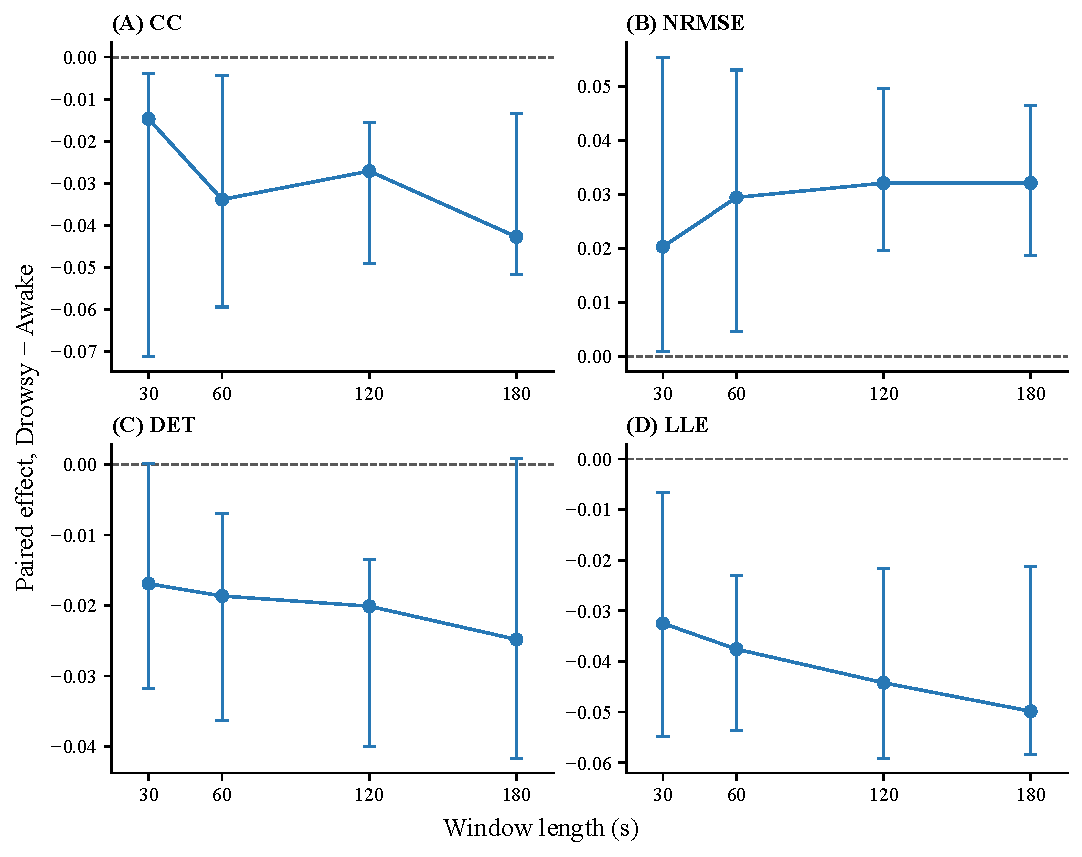
\includegraphics[width=\linewidth,height=.75\textheight,keepaspectratio]{figures/figure_S07.pdf}
\caption{Window-length sensitivity. Median paired effects and 95\% percentile bootstrap CIs for Mean CC, Mean NRMSE, DET, and LLE at 30, 60, 120, and 180 s. Median directions are preserved, while magnitude and uncertainty vary; DET intervals include zero at 30 and 180 s. Each duration has 20 paired sessions, with fewer eligible windows at longer durations and additional LLE fit screening (Table~\ref{tab:supp_window}).}\label{fig:supp_window}
\end{figure}
\subsection{Label Sensitivity}\label{sec:supp_11}
P0 used primary recorded labels. T30/T60 excluded samples within $\pm$30/$\pm$60 s of transitions, while S3/S5 retained same-state episodes lasting at least 180/300 s. Windows were constructed and screened under each rule; cohorts need not be nested subsets of P0. General-QC retention is in Table~\ref{tab:supp_label}A. P0/T30/T60/S3 retained 20 paired sessions and S5 retained 19; LLE additionally used fit acceptance.

All 16 alternative-rule median effects preserved the four headline directions and had $q_{\mathrm{BH}}<0.05$ within each rule’s BH4 family (Table~\ref{tab:supp_label}B; Fig.~\ref{fig:supp_label}). Magnitudes differed. The T60 Mean CC CI $[-0.0561,+0.0059]$ and T30 LLE CI $[-0.0535,+0.0020]$ included zero, consistent with the CI/test distinction in Section~\ref{sec:supp_9}. P0 remains the fixed primary reference, with BH7 rather than alternative-rule BH4 correction.

\begingroup\small
\setlength{\tabcolsep}{3pt}
\renewcommand{\arraystretch}{1.18}
\stepcounter{supptablepanel}
\begin{longtable}{L{\dimexpr0.09195\linewidth-1.10345\tabcolsep\relax}L{\dimexpr0.45977\linewidth-5.51724\tabcolsep\relax}L{\dimexpr0.11494\linewidth-1.37931\tabcolsep\relax}L{\dimexpr0.11494\linewidth-1.37931\tabcolsep\relax}L{\dimexpr0.11494\linewidth-1.37931\tabcolsep\relax}L{\dimexpr0.10345\linewidth-1.24138\tabcolsep\relax}}
\caption{Label definitions, retained cohorts, and four-metric effects.}\label{tab:supp_label}\\
\multicolumn{6}{l}{\textbf{Panel A. Rule definitions and general-QC retention}}\\
\toprule
Rule & Definition & Awake windows & Drowsy windows & Total windows & Paired n\\
\midrule\endfirsthead
\multicolumn{6}{l}{Table~\ref{tab:supp_label} (continued)}\\
\toprule
Rule & Definition & Awake windows & Drowsy windows & Total windows & Paired n\\
\midrule\endhead
\bottomrule\endfoot
\bottomrule\endlastfoot
P0 & Primary recorded labels & 596 & 305 & 901 & 20\\
T30 & Exclude samples within $\pm$30 s of transitions & 586 & 274 & 860 & 20\\
T60 & Exclude samples within $\pm$60 s of transitions & 551 & 236 & 787 & 20\\
S3 & Retain same-state episodes $\geq$180 s & 609 & 291 & 900 & 20\\
S5 & Retain same-state episodes $\geq$300 s & 581 & 265 & 846 & 19\\
\end{longtable}
\endgroup
\begin{landscape}
\begingroup\small
\setlength{\tabcolsep}{3pt}
\renewcommand{\arraystretch}{1.18}
\addtocounter{table}{-1}
\stepcounter{supptablepanel}
\begin{longtable}{L{\dimexpr0.06154\linewidth-1.23077\tabcolsep\relax}L{\dimexpr0.12308\linewidth-2.46154\tabcolsep\relax}L{\dimexpr0.13077\linewidth-2.61538\tabcolsep\relax}L{\dimexpr0.06154\linewidth-1.23077\tabcolsep\relax}L{\dimexpr0.09231\linewidth-1.84615\tabcolsep\relax}L{\dimexpr0.19231\linewidth-3.84615\tabcolsep\relax}L{\dimexpr0.09231\linewidth-1.84615\tabcolsep\relax}L{\dimexpr0.08462\linewidth-1.69231\tabcolsep\relax}L{\dimexpr0.07692\linewidth-1.53846\tabcolsep\relax}L{\dimexpr0.08462\linewidth-1.69231\tabcolsep\relax}}
\multicolumn{10}{l}{Table~\ref{tab:supp_label} (continued)}\\
\multicolumn{10}{l}{\textbf{Panel B. Four-metric inference}}\\
\toprule
Rule & Family & Metric & Paired n & Median $\Delta$ & 95\% CI & Raw $p$ & $q_{\mathrm{BH}}$ & $r_{\mathrm{rb}}$ & Direction count\\
\midrule\endfirsthead
\multicolumn{10}{l}{Table~\ref{tab:supp_label} (continued)}\\
\toprule
Rule & Family & Metric & Paired n & Median $\Delta$ & 95\% CI & Raw $p$ & $q_{\mathrm{BH}}$ & $r_{\mathrm{rb}}$ & Direction count\\
\midrule\endhead
\bottomrule\endfoot
\bottomrule\endlastfoot
P0 & \textbf{Primary BH7} & Mean CC & 20 & -0.0339 & [-0.0595, -0.0043] & 0.02148438 & 0.0376 & -0.581 & 15/\allowbreak 20\\
P0 & \textbf{Primary BH7} & Mean NRMSE & 20 & +0.0294 & [0.0047, 0.0530] & 0.00729561 & 0.0255 & +0.667 & 15/\allowbreak 20\\
P0 & \textbf{Primary BH7} & DET & 20 & -0.0186 & [-0.0364, -0.0069] & 0.02148438 & 0.0376 & -0.581 & 15/\allowbreak 20\\
P0 & \textbf{Primary BH7} & LLE & 20 & -0.0376 & [-0.0537, -0.0230] & 0.00070763 & 0.0050 & -0.810 & 16/\allowbreak 20\\
T30 & Sensitivity BH4 & Mean CC & 20 & -0.0482 & [-0.0689, -0.0152] & 0.0048599 & 0.0097 & -0.695 & 17/\allowbreak 20\\
T30 & Sensitivity BH4 & Mean NRMSE & 20 & +0.0406 & [+0.0190, +0.0570] & 0.0031528 & 0.0097 & +0.724 & 16/\allowbreak 20\\
T30 & Sensitivity BH4 & DET & 20 & -0.0183 & [-0.0332, -0.0011] & 0.0083084 & 0.0111 & -0.657 & 14/\allowbreak 20\\
T30 & Sensitivity BH4 & LLE & 20 & -0.0322 & [-0.0535, +0.0020] & 0.021484 & 0.0215 & -0.581 & 14/\allowbreak 20\\
T60 & Sensitivity BH4 & Mean CC & 20 & -0.0251 & [-0.0561, +0.0059] & 0.039989 & 0.0400 & -0.524 & 13/\allowbreak 20\\
T60 & Sensitivity BH4 & Mean NRMSE & 20 & +0.0278 & [+0.0027, +0.0479] & 0.013617 & 0.0256 & +0.619 & 14/\allowbreak 20\\
T60 & Sensitivity BH4 & DET & 20 & -0.0167 & [-0.0294, -0.0066] & 0.019234 & 0.0256 & -0.590 & 15/\allowbreak 20\\
T60 & Sensitivity BH4 & LLE & 20 & -0.0393 & [-0.0636, -0.0075] & 0.0023251 & 0.0093 & -0.743 & 15/\allowbreak 20\\
S3 & Sensitivity BH4 & Mean CC & 20 & -0.0361 & [-0.0548, -0.0033] & 0.010689 & 0.0136 & -0.638 & 14/\allowbreak 20\\
S3 & Sensitivity BH4 & Mean NRMSE & 20 & +0.0357 & [+0.0032, +0.0457] & 0.0063896 & 0.0128 & +0.676 & 15/\allowbreak 20\\
S3 & Sensitivity BH4 & DET & 20 & -0.0189 & [-0.0326, -0.0069] & 0.013617 & 0.0136 & -0.619 & 15/\allowbreak 20\\
S3 & Sensitivity BH4 & LLE & 20 & -0.0344 & [-0.0495, -0.0104] & 0.0010166 & 0.0041 & -0.790 & 15/\allowbreak 20\\
S5 & Sensitivity BH4 & Mean CC & 19 & -0.0337 & [-0.0495, -0.0077] & 0.01236 & 0.0141 & -0.642 & 14/\allowbreak 19\\
S5 & Sensitivity BH4 & Mean NRMSE & 19 & +0.0367 & [+0.0056, +0.0504] & 0.0045776 & 0.0092 & +0.716 & 16/\allowbreak 19\\
S5 & Sensitivity BH4 & DET & 19 & -0.0213 & [-0.0305, -0.0049] & 0.014069 & 0.0141 & -0.632 & 15/\allowbreak 19\\
S5 & Sensitivity BH4 & LLE & 19 & -0.0321 & [-0.0499, -0.0147] & 0.0014114 & 0.0056 & -0.789 & 14/\allowbreak 19\\
\end{longtable}
\endgroup
{\small Panel A retention precedes LLE fit screening. In Panel B the Family column distinguishes primary BH7 reference rows from BH4 sensitivity rows; correction is never pooled across rules.}\par
{\small Direction counts are decreases for Mean CC/DET/LLE and increases for Mean NRMSE. Effect/CI units are s$^{-1}$ for LLE and dimensionless otherwise. Raw p retains source precision; alternative-rule q is shown to four decimals.}\par
\end{landscape}
\begin{figure}[p]
\centering
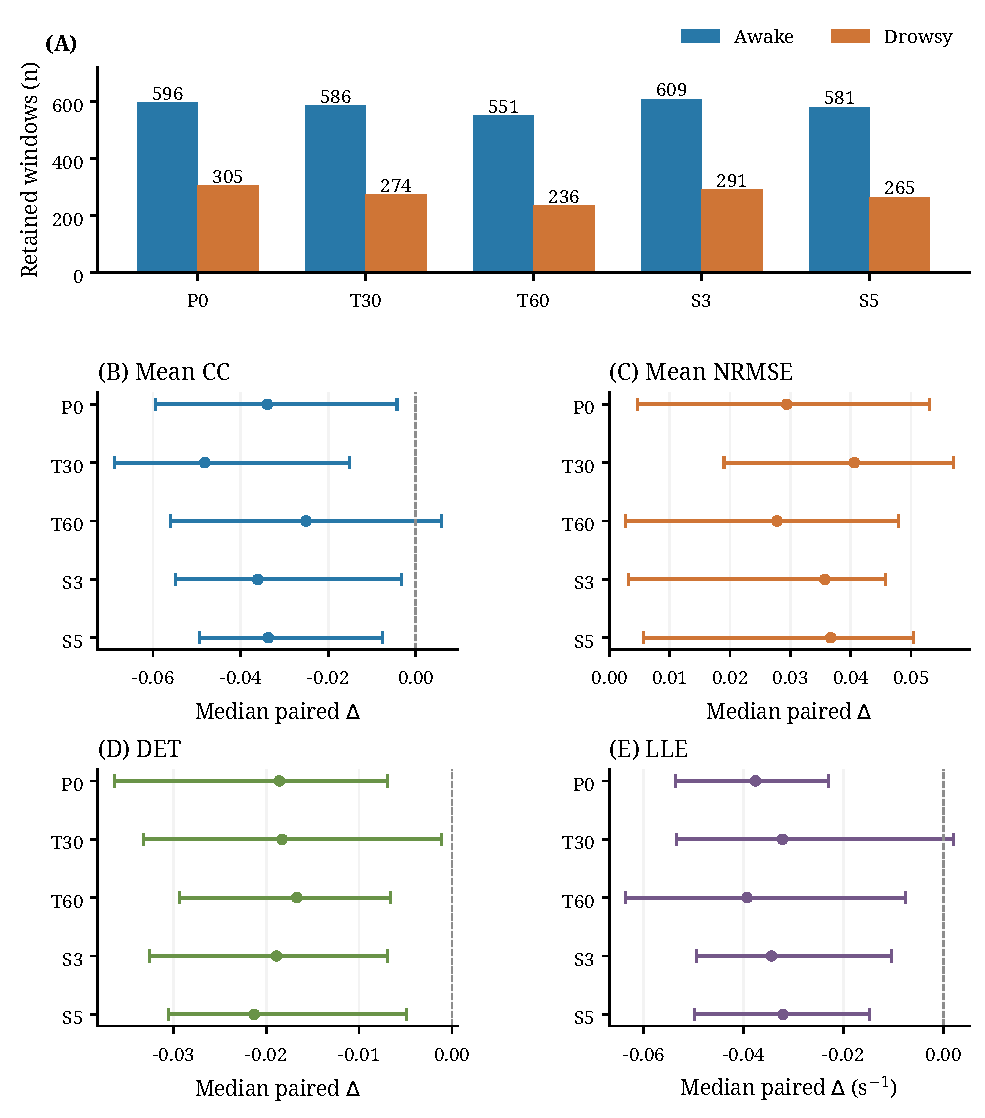
\includegraphics[width=\linewidth,height=.75\textheight,keepaspectratio]{figures/figure_S08.pdf}
\caption{Label sensitivity. (A) Awake/Drowsy general-QC retention under P0/T30/T60/S3/S5. (B--E) Four-metric median paired effects and 95\% percentile CIs, using Table~\ref{tab:supp_primary} for P0 and alternative-rule summaries for sensitivities. Paired n is 20 except S5 (19). Median directions are preserved; T60 Mean CC and T30 LLE CIs include zero. Alternative-rule support uses BH4 within rule; P0 retains primary BH7.}\label{fig:supp_label}
\end{figure}
\subsection{Reconstruction and Estimator Sensitivity}\label{sec:supp_12}
One reconstruction or estimator setting was perturbed at a time, retaining nominal choices for other settings. These analyses describe dependence within the tested configurations.

\subsubsection{Embedding Delay and Dimension}\label{sec:supp_12_1}
Delay sensitivity used $\tau=0.12,0.16,0.20$ s at $m=8$; dimension sensitivity used $m=7,8,9$ at $\tau=0.16$ s (Table~\ref{tab:supp_reconstruction}). Mean CC, Mean NRMSE, and LLE retained negative, positive, and negative median effects across delays. DET was delay-sensitive: its nominal $-0.0186$ became near-zero and positive at 0.12 s ($+0.0025$) and 0.20 s ($+0.0015$). Both non-nominal CIs spanned zero and lacked BH support.

All four median directions were preserved across $m=7$--9, but magnitudes varied, including LLE. DET lacked BH4 support at $m=7$ ($q=0.053169$) and $m=9$ ($q=0.058258$), despite negative effects and CIs excluding zero. Some Mean CC/NRMSE CIs also spanned zero. Table~\ref{tab:supp_reconstruction} distinguishes nominal primary BH7 rows from alternative-setting BH4 rows; no correction is pooled across settings. DET is therefore not uniformly stable to embedding delay.

\begin{landscape}
\begingroup\small
\setlength{\tabcolsep}{3pt}
\renewcommand{\arraystretch}{1.18}
\stepcounter{supptablepanel}
\begin{longtable}{L{\dimexpr0.07519\linewidth-1.50376\tabcolsep\relax}L{\dimexpr0.12030\linewidth-2.40602\tabcolsep\relax}L{\dimexpr0.12782\linewidth-2.55639\tabcolsep\relax}L{\dimexpr0.06767\linewidth-1.35338\tabcolsep\relax}L{\dimexpr0.09023\linewidth-1.80451\tabcolsep\relax}L{\dimexpr0.18797\linewidth-3.75940\tabcolsep\relax}L{\dimexpr0.09023\linewidth-1.80451\tabcolsep\relax}L{\dimexpr0.08271\linewidth-1.65414\tabcolsep\relax}L{\dimexpr0.07519\linewidth-1.50376\tabcolsep\relax}L{\dimexpr0.08271\linewidth-1.65414\tabcolsep\relax}}
\caption{Reconstruction sensitivity with explicit correction families.}\label{tab:supp_reconstruction}\\
\multicolumn{10}{l}{\textbf{Panel A. Delay sensitivity at m=8}}\\
\toprule
Setting & Family & Metric & Paired n & Median $\Delta$ & 95\% CI & Raw $p$ & $q_{\mathrm{BH}}$ & $r_{\mathrm{rb}}$ & Direction count\\
\midrule\endfirsthead
\multicolumn{10}{l}{Table~\ref{tab:supp_reconstruction} (continued)}\\
\toprule
Setting & Family & Metric & Paired n & Median $\Delta$ & 95\% CI & Raw $p$ & $q_{\mathrm{BH}}$ & $r_{\mathrm{rb}}$ & Direction count\\
\midrule\endhead
\bottomrule\endfoot
\bottomrule\endlastfoot
0.12 & Sensitivity BH4 & Mean CC & 20 & -0.0317 & [-0.0522, +0.0094] & 0.036234 & 0.048312 & -0.533 & 13/\allowbreak 20\\
0.12 & Sensitivity BH4 & Mean NRMSE & 20 & +0.0321 & [-0.0042, +0.0492] & 0.029575 & 0.048312 & +0.552 & 13/\allowbreak 20\\
0.12 & Sensitivity BH4 & DET & 20 & +0.0025 & [-0.0078, +0.0076] & 0.784126 & 0.784126 & +0.076 & 7/\allowbreak 20\\
0.12 & Sensitivity BH4 & LLE & 20 & -0.0361 & [-0.0567, +0.0042] & 0.017181 & 0.048312 & -0.600 & 14/\allowbreak 20\\
0.16 & \textbf{Primary BH7} & Mean CC & 20 & -0.0339 & [-0.0595, -0.0043] & 0.02148438 & 0.0376 & -0.581 & 15/\allowbreak 20\\
0.16 & \textbf{Primary BH7} & Mean NRMSE & 20 & +0.0294 & [0.0047, 0.0530] & 0.00729561 & 0.0255 & +0.667 & 15/\allowbreak 20\\
0.16 & \textbf{Primary BH7} & DET & 20 & -0.0186 & [-0.0364, -0.0069] & 0.02148438 & 0.0376 & -0.581 & 15/\allowbreak 20\\
0.16 & \textbf{Primary BH7} & LLE & 20 & -0.0376 & [-0.0537, -0.0230] & 0.00070763 & 0.0050 & -0.810 & 16/\allowbreak 20\\
0.20 & Sensitivity BH4 & Mean CC & 20 & -0.0316 & [-0.0529, -0.0008] & 0.015312 & 0.020416 & -0.610 & 14/\allowbreak 20\\
0.20 & Sensitivity BH4 & Mean NRMSE & 20 & +0.0296 & [+0.0056, +0.0476] & 0.005581 & 0.011162 & +0.686 & 16/\allowbreak 20\\
0.20 & Sensitivity BH4 & DET & 20 & +0.0015 & [-0.0099, +0.0148] & 0.985435 & 0.985435 & +0.010 & 10/\allowbreak 20\\
0.20 & Sensitivity BH4 & LLE & 20 & -0.0464 & [-0.0572, -0.0240] & 0.000036 & 0.000145 & -0.933 & 17/\allowbreak 20\\
\end{longtable}
\clearpage
\addtocounter{table}{-1}
\stepcounter{supptablepanel}
\begin{longtable}{L{\dimexpr0.07519\linewidth-1.50376\tabcolsep\relax}L{\dimexpr0.12030\linewidth-2.40602\tabcolsep\relax}L{\dimexpr0.12782\linewidth-2.55639\tabcolsep\relax}L{\dimexpr0.06767\linewidth-1.35338\tabcolsep\relax}L{\dimexpr0.09023\linewidth-1.80451\tabcolsep\relax}L{\dimexpr0.18797\linewidth-3.75940\tabcolsep\relax}L{\dimexpr0.09023\linewidth-1.80451\tabcolsep\relax}L{\dimexpr0.08271\linewidth-1.65414\tabcolsep\relax}L{\dimexpr0.07519\linewidth-1.50376\tabcolsep\relax}L{\dimexpr0.08271\linewidth-1.65414\tabcolsep\relax}}
\multicolumn{10}{l}{Table~\ref{tab:supp_reconstruction} (continued)}\\
\multicolumn{10}{l}{\textbf{Panel B. Dimension sensitivity at delay 0.16 s}}\\
\toprule
Setting & Family & Metric & Paired n & Median $\Delta$ & 95\% CI & Raw $p$ & $q_{\mathrm{BH}}$ & $r_{\mathrm{rb}}$ & Direction count\\
\midrule\endfirsthead
\multicolumn{10}{l}{Table~\ref{tab:supp_reconstruction} (continued)}\\
\toprule
Setting & Family & Metric & Paired n & Median $\Delta$ & 95\% CI & Raw $p$ & $q_{\mathrm{BH}}$ & $r_{\mathrm{rb}}$ & Direction count\\
\midrule\endhead
\bottomrule\endfoot
\bottomrule\endlastfoot
7 & Sensitivity BH4 & Mean CC & 20 & -0.0307 & [-0.0565, +0.0045] & 0.026642 & 0.035522 & -0.562 & 13/\allowbreak 20\\
7 & Sensitivity BH4 & Mean NRMSE & 20 & +0.0377 & [-0.0023, +0.0561] & 0.023951 & 0.035522 & +0.571 & 13/\allowbreak 20\\
7 & Sensitivity BH4 & DET & 20 & -0.0145 & [-0.0303, -0.0047] & 0.053169 & 0.053169 & -0.495 & 15/\allowbreak 20\\
7 & Sensitivity BH4 & LLE & 20 & -0.0285 & [-0.0549, -0.0076] & 0.004860 & 0.019440 & -0.695 & 16/\allowbreak 20\\
8 & \textbf{Primary BH7} & Mean CC & 20 & -0.0339 & [-0.0595, -0.0043] & 0.02148438 & 0.0376 & -0.581 & 15/\allowbreak 20\\
8 & \textbf{Primary BH7} & Mean NRMSE & 20 & +0.0294 & [0.0047, 0.0530] & 0.00729561 & 0.0255 & +0.667 & 15/\allowbreak 20\\
8 & \textbf{Primary BH7} & DET & 20 & -0.0186 & [-0.0364, -0.0069] & 0.02148438 & 0.0376 & -0.581 & 15/\allowbreak 20\\
8 & \textbf{Primary BH7} & LLE & 20 & -0.0376 & [-0.0537, -0.0230] & 0.00070763 & 0.0050 & -0.810 & 16/\allowbreak 20\\
9 & Sensitivity BH4 & Mean CC & 20 & -0.0251 & [-0.0492, +0.0055] & 0.029575 & 0.039434 & -0.552 & 13/\allowbreak 20\\
9 & Sensitivity BH4 & Mean NRMSE & 20 & +0.0315 & [+0.0043, +0.0483] & 0.008308 & 0.016617 & +0.657 & 15/\allowbreak 20\\
9 & Sensitivity BH4 & DET & 20 & -0.0200 & [-0.0321, -0.0052] & 0.058258 & 0.058258 & -0.486 & 15/\allowbreak 20\\
9 & Sensitivity BH4 & LLE & 20 & -0.0247 & [-0.0534, -0.0102] & 0.000586 & 0.002342 & -0.819 & 16/\allowbreak 20\\
\end{longtable}
\endgroup
{\small Panel A settings are delay in seconds; Panel B settings are dimension. Primary BH7 rows reproduce Table~\ref{tab:supp_primary}, while sensitivity BH4 rows use the four-metric family within each alternative setting.}\par
{\small Direction counts follow nominal expected signs (Mean CC/DET/LLE decrease; Mean NRMSE increase), including when aggregate DET reverses. Effects/CIs use manuscript precision and units; alternative p/q retains six-decimal source precision. This is a one-factor analysis, not a full factorial grid.}\par
\end{landscape}
\subsubsection{RQA Estimator Settings}\label{sec:supp_12_2}
RQA sensitivity tested $\mathrm{RR}=0.01,0.02,0.03$ and Theiler multipliers 0.75, 1.00, 1.25 relative to nominal $W=(m-1)d$. All settings retained 901 windows and 20 paired sessions. Table~\ref{tab:supp_estimator}A reports available DET/LAM/TT inference with raw p only. DET remained negative across these settings, although at RR=0.01 its CI spanned zero and p was 0.082550. Direction stability under these RQA choices contrasts with delay-dependent sign reversal in Section~\ref{sec:supp_12_1}.

LAM/TT remained secondary: all median effects were positive, all CIs spanned zero, and all raw p values exceeded 0.05. $L_{\mathrm{mean}}$ estimator sensitivity was not available. Metric interpretation follows Section~\ref{sec:supp_6}.

\subsubsection{LLE Estimator Settings}\label{sec:supp_12_3}
LLE sensitivity tested fit intervals 0.60--1.10, 0.80--1.30 (nominal), and 1.00--1.50 s; $R^2$ thresholds 0.90/0.95; and Theiler multipliers 0.75/1.00/1.25 relative to its spectral-mean-period exclusion (Section~\ref{sec:supp_7}). All settings retained 20 paired sessions. Every median effect was negative, every CI excluded zero, and raw p was below 0.05 (Table~\ref{tab:supp_estimator}B). No BH correction was applied across estimator settings.

Fit intervals retained 802/872/889 of 901 input windows, respectively. Increasing $R^2$ from 0.90 to 0.95 retained 734 rather than 872 windows and reduced the median decrease. The 0.75/1.00 Theiler multipliers gave the same effect and retention; 1.25 retained 874 windows and changed magnitude. Direction preservation therefore coexists with magnitude and cohort changes; the estimator is not parameter-independent.

\begin{landscape}
\begingroup\small
\setlength{\tabcolsep}{3pt}
\renewcommand{\arraystretch}{1.18}
\stepcounter{supptablepanel}
\begin{longtable}{L{\dimexpr0.13534\linewidth-2.70677\tabcolsep\relax}L{\dimexpr0.06767\linewidth-1.35338\tabcolsep\relax}L{\dimexpr0.07519\linewidth-1.50376\tabcolsep\relax}L{\dimexpr0.07519\linewidth-1.50376\tabcolsep\relax}L{\dimexpr0.06015\linewidth-1.20301\tabcolsep\relax}L{\dimexpr0.10526\linewidth-2.10526\tabcolsep\relax}L{\dimexpr0.20301\linewidth-4.06015\tabcolsep\relax}L{\dimexpr0.09023\linewidth-1.80451\tabcolsep\relax}L{\dimexpr0.09023\linewidth-1.80451\tabcolsep\relax}L{\dimexpr0.09774\linewidth-1.95489\tabcolsep\relax}}
\caption{RQA and LLE estimator sensitivity.}\label{tab:supp_estimator}\\
\multicolumn{10}{l}{\textbf{Panel A. RQA RR and Theiler settings}}\\
\toprule
Factor & Setting & Metric & Valid windows & Paired n & Median $\Delta$ & 95\% CI & Raw $p$ & $r_{\mathrm{rb}}$ & Direction count\\
\midrule\endfirsthead
\multicolumn{10}{l}{Table~\ref{tab:supp_estimator} (continued)}\\
\toprule
Factor & Setting & Metric & Valid windows & Paired n & Median $\Delta$ & 95\% CI & Raw $p$ & $r_{\mathrm{rb}}$ & Direction count\\
\midrule\endhead
\bottomrule\endfoot
\bottomrule\endlastfoot
RR & 0.01 & DET & 901 & 20 & -0.015214 & [-0.033764, +0.002064] & 0.082550 & -0.447619 & 14/\allowbreak 20\\
RR & 0.01 & LAM & 901 & 20 & 0.014242 & [-0.005819, +0.057725] & 0.132727 & 0.390476 & 13/\allowbreak 20\\
RR & 0.01 & TT & 901 & 20 & 0.000343 & [-0.000043, +0.004808] & 0.214602 & 0.352941 & 10/\allowbreak 20; 4 zero\\
RR & 0.02 & DET & 901 & 20 & -0.0186 & [-0.0364, -0.0069] & 0.021484 & -0.581 & 15/\allowbreak 20\\
RR & 0.02 & LAM & 901 & 20 & +0.0165 & [-0.0044, 0.0635] & 0.142906 & +0.381 & 13/\allowbreak 20\\
RR & 0.02 & TT & 901 & 20 & +0.0095 & [-0.0034, 0.0160] & 0.202450 & +0.333 & 14/\allowbreak 20\\
RR & 0.03 & DET & 901 & 20 & -0.017813 & [-0.033859, -0.007863] & 0.021484 & -0.580952 & 15/\allowbreak 20\\
RR & 0.03 & LAM & 901 & 20 & 0.020281 & [-0.005463, +0.051395] & 0.082550 & 0.447619 & 13/\allowbreak 20\\
RR & 0.03 & TT & 901 & 20 & 0.022063 & [-0.007639, +0.033264] & 0.294252 & 0.276190 & 14/\allowbreak 20\\
Theiler multiplier & 0.75 & DET & 901 & 20 & -0.019191 & [-0.036836, -0.006809] & 0.021484 & -0.580952 & 15/\allowbreak 20\\
Theiler multiplier & 0.75 & LAM & 901 & 20 & 0.019785 & [-0.003072, +0.062855] & 0.123093 & 0.400000 & 13/\allowbreak 20\\
Theiler multiplier & 0.75 & TT & 901 & 20 & 0.009809 & [-0.003114, +0.015962] & 0.189348 & 0.342857 & 14/\allowbreak 20\\
Theiler multiplier & 1.00 & DET & 901 & 20 & -0.0186 & [-0.0364, -0.0069] & 0.021484 & -0.581 & 15/\allowbreak 20\\
Theiler multiplier & 1.00 & LAM & 901 & 20 & +0.0165 & [-0.0044, 0.0635] & 0.142906 & +0.381 & 13/\allowbreak 20\\
Theiler multiplier & 1.00 & TT & 901 & 20 & +0.0095 & [-0.0034, 0.0160] & 0.202450 & +0.333 & 14/\allowbreak 20\\
Theiler multiplier & 1.25 & DET & 901 & 20 & -0.019033 & [-0.037873, -0.007730] & 0.017181 & -0.600000 & 15/\allowbreak 20\\
Theiler multiplier & 1.25 & LAM & 901 & 20 & 0.019372 & [-0.005161, +0.062616] & 0.132727 & 0.390476 & 12/\allowbreak 20\\
Theiler multiplier & 1.25 & TT & 901 & 20 & 0.009844 & [-0.002347, +0.017601] & 0.176853 & 0.352381 & 14/\allowbreak 20\\
\end{longtable}
\clearpage
\addtocounter{table}{-1}
\stepcounter{supptablepanel}
\begin{longtable}{L{\dimexpr0.10526\linewidth-2.31579\tabcolsep\relax}L{\dimexpr0.10877\linewidth-2.39298\tabcolsep\relax}L{\dimexpr0.07719\linewidth-1.69825\tabcolsep\relax}L{\dimexpr0.06316\linewidth-1.38947\tabcolsep\relax}L{\dimexpr0.06316\linewidth-1.38947\tabcolsep\relax}L{\dimexpr0.05614\linewidth-1.23509\tabcolsep\relax}L{\dimexpr0.09123\linewidth-2.00702\tabcolsep\relax}L{\dimexpr0.18947\linewidth-4.16842\tabcolsep\relax}L{\dimexpr0.08421\linewidth-1.85263\tabcolsep\relax}L{\dimexpr0.08421\linewidth-1.85263\tabcolsep\relax}L{\dimexpr0.07719\linewidth-1.69825\tabcolsep\relax}}
\multicolumn{11}{l}{Table~\ref{tab:supp_estimator} (continued)}\\
\multicolumn{11}{l}{\textbf{Panel B. LLE fit, quality, and Theiler settings}}\\
\toprule
Factor & Setting & Passing /\allowbreak  input & Awake windows & Drowsy windows & Paired n & Median $\Delta$ & 95\% CI & Raw $p$ & $r_{\mathrm{rb}}$ & Decrease count\\
\midrule\endfirsthead
\multicolumn{11}{l}{Table~\ref{tab:supp_estimator} (continued)}\\
\toprule
Factor & Setting & Passing /\allowbreak  input & Awake windows & Drowsy windows & Paired n & Median $\Delta$ & 95\% CI & Raw $p$ & $r_{\mathrm{rb}}$ & Decrease count\\
\midrule\endhead
\bottomrule\endfoot
\bottomrule\endlastfoot
Fit interval (s) & 0.60--1.10 & 802/\allowbreak 901 & 542 & 260 & 20 & -0.034980 & [-0.064607, -0.019121] & 0.000261 & -0.857143 & 18/\allowbreak 20\\
Fit interval (s) & 0.80--1.30 & 872/\allowbreak 901 & 579 & 293 & 20 & -0.0376 & [-0.0537, -0.0230] & 0.000708 & -0.810 & 16/\allowbreak 20\\
Fit interval (s) & 1.00--1.50 & 889/\allowbreak 901 & 588 & 301 & 20 & -0.030357 & [-0.045778, -0.003941] & 0.008308 & -0.657143 & 15/\allowbreak 20\\
$R^2$ threshold & 0.90 & 872/\allowbreak 901 & 579 & 293 & 20 & -0.0376 & [-0.0537, -0.0230] & 0.000708 & -0.810 & 16/\allowbreak 20\\
$R^2$ threshold & 0.95 & 734/\allowbreak 901 & 500 & 234 & 20 & -0.030618 & [-0.041701, -0.013987] & 0.002325 & -0.742857 & 16/\allowbreak 20\\
Theiler multiplier & 0.75 & 872/\allowbreak 901 & 579 & 293 & 20 & -0.037570 & [-0.053698, -0.022976] & 0.000708 & -0.809524 & 16/\allowbreak 20\\
Theiler multiplier & 1.00 & 872/\allowbreak 901 & 579 & 293 & 20 & -0.0376 & [-0.0537, -0.0230] & 0.000708 & -0.810 & 16/\allowbreak 20\\
Theiler multiplier & 1.25 & 874/\allowbreak 901 & 580 & 294 & 20 & -0.029763 & [-0.056095, -0.016331] & 0.002325 & -0.742857 & 16/\allowbreak 20\\
\end{longtable}
\endgroup
{\small Both panels report raw p only, with no BH correction across settings. Paired n is 20 throughout. Panel A counts decreases for DET and increases for LAM/TT; RR=0.01 TT has four zero differences removed before rank calculations. DET/LAM are dimensionless and TT uses sample-index line lengths.}\par
{\small Panel B passing counts use the 901 input-window denominator; effects/CIs are in s$^{-1}$. Theiler multipliers use each estimator’s own nominal exclusion. Nominal effects/CIs/$r_{\mathrm{rb}}$ reproduce Table~\ref{tab:supp_primary} at manuscript precision; perturbation values retain six decimals.}\par
\end{landscape}
\subsection{Unknown Repeated-Session Dependence}\label{sec:supp_13}
To assess the linkage limitation in Section~\ref{sec:supp_1}, a hypothetical dependence analysis grouped 20 sessions into 10 two-session clusters using random perfect matchings. Sampling with replacement paired adjacent entries in random permutations, producing 100,000 sampled matchings and 99,990 unique matchings among 654,729,075 theoretically possible matchings. These clusters do not recover participant identity or establish actual session independence.

For each matching, cluster differences were arithmetic means of the two session differences; the effect was the median of 10 cluster differences. Conditional two-sided signed-rank tests discarded differences within $10^{-12}$ of zero and averaged ranks for absolute-value ties. BH correction covered seven metrics within each matching, without nested bootstrap. Table~\ref{tab:supp_repeated}A gives matching-distribution percentiles, not bootstrap CIs.

All four headline median directions were preserved in every sampled matching. Fractions with $q_{\mathrm{BH}}<0.05$ were 19.36\% (Mean CC), 27.82\% (Mean NRMSE), 22.59\% (DET), and 79.69\% (LLE). Direction was more stable than support after reducing effective units to 10 hypothetical clusters; LLE retained the strongest support within this analysis. Frequencies describe the specified hypothetical matching design, not probabilities that the true result is significant. They do not provide participant-level inference. Cumulative 50,000/100,000-draw summaries were similar (Table~\ref{tab:supp_repeated}B; Fig.~\ref{fig:supp_repeated}), supporting Monte Carlo stability without resolving linkage.

\begin{landscape}
\begingroup\small
\setlength{\tabcolsep}{3pt}
\renewcommand{\arraystretch}{1.18}
\stepcounter{supptablepanel}
\begin{longtable}{L{\dimexpr0.16162\linewidth-1.93939\tabcolsep\relax}L{\dimexpr0.13131\linewidth-1.57576\tabcolsep\relax}L{\dimexpr0.14141\linewidth-1.69697\tabcolsep\relax}L{\dimexpr0.14141\linewidth-1.69697\tabcolsep\relax}L{\dimexpr0.15152\linewidth-1.81818\tabcolsep\relax}L{\dimexpr0.27273\linewidth-3.27273\tabcolsep\relax}}
\caption{Hypothetical matching distributions and convergence.}\label{tab:supp_repeated}\\
\multicolumn{6}{l}{\textbf{Panel A. Hypothetical matching distribution, 100,000 draws}}\\
\toprule
Metric & Nominal direction & Sign preserved (\%) & $q_{\mathrm{BH}}<0.05$ (\%) & Median matching $\Delta$ & 2.5th--97.5th percentile range\\
\midrule\endfirsthead
\multicolumn{6}{l}{Table~\ref{tab:supp_repeated} (continued)}\\
\toprule
Metric & Nominal direction & Sign preserved (\%) & $q_{\mathrm{BH}}<0.05$ (\%) & Median matching $\Delta$ & 2.5th--97.5th percentile range\\
\midrule\endhead
\bottomrule\endfoot
\bottomrule\endlastfoot
Mean CC & Decrease & 100.00 & 19.36 & -0.0242 & [-0.0359, -0.0147]\\
Mean NRMSE & Increase & 100.00 & 27.82 & +0.0263 & [+0.0185, +0.0343]\\
DET & Decrease & 100.00 & 22.59 & -0.0181 & [-0.0255, -0.0100]\\
$L_{\mathrm{mean}}$ & Decrease & 100.00 & 2.41 & -0.0657 & [-0.1000, -0.0333]\\
LAM & Increase & 99.63 & 2.94 & +0.0227 & [+0.0063, +0.0402]\\
TT & Increase & 99.25 & 0.04 & +0.0076 & [+0.0012, +0.0137]\\
LLE & Decrease & 100.00 & 79.69 & -0.0356 & [-0.0446, -0.0266]\\
\end{longtable}
\addtocounter{table}{-1}
\stepcounter{supptablepanel}
\begin{longtable}{L{\dimexpr0.16162\linewidth-1.93939\tabcolsep\relax}L{\dimexpr0.13131\linewidth-1.57576\tabcolsep\relax}L{\dimexpr0.14141\linewidth-1.69697\tabcolsep\relax}L{\dimexpr0.14141\linewidth-1.69697\tabcolsep\relax}L{\dimexpr0.15152\linewidth-1.81818\tabcolsep\relax}L{\dimexpr0.27273\linewidth-3.27273\tabcolsep\relax}}
\multicolumn{6}{l}{\textbf{Panel B. Cumulative Monte Carlo summaries}}\\
\toprule
Draws & Metric & Sign preserved (\%) & $q_{\mathrm{BH}}<0.05$ (\%) & Median matching $\Delta$ & 2.5th--97.5th percentile range\\
\midrule\endfirsthead
\multicolumn{6}{l}{Table~\ref{tab:supp_repeated} (continued)}\\
\toprule
Draws & Metric & Sign preserved (\%) & $q_{\mathrm{BH}}<0.05$ (\%) & Median matching $\Delta$ & 2.5th--97.5th percentile range\\
\midrule\endhead
\bottomrule\endfoot
\bottomrule\endlastfoot
50000 & Mean CC & 100.00 & 19.44 & -0.0242 & [-0.0360, -0.0147]\\
50000 & Mean NRMSE & 100.00 & 27.94 & +0.0263 & [+0.0185, +0.0342]\\
50000 & DET & 100.00 & 22.69 & -0.0181 & [-0.0256, -0.0100]\\
50000 & LLE & 100.00 & 79.69 & -0.0356 & [-0.0446, -0.0266]\\
100000 & Mean CC & 100.00 & 19.36 & -0.0242 & [-0.0359, -0.0147]\\
100000 & Mean NRMSE & 100.00 & 27.82 & +0.0263 & [+0.0185, +0.0343]\\
100000 & DET & 100.00 & 22.59 & -0.0181 & [-0.0255, -0.0100]\\
100000 & LLE & 100.00 & 79.69 & -0.0356 & [-0.0446, -0.0266]\\
\end{longtable}
\endgroup
{\small Sign preservation compares each matching’s median cluster effect with the nominal direction. q support uses BH7 within matching. Ranges are 2.5th--97.5th percentiles of the hypothetical matching distribution, not bootstrap CIs or participant-effect intervals. Units follow Table~\ref{tab:supp_primary}.}\par
{\small The 50k/100k rows are cumulative prefixes of the same sequence, not independent runs. No participant mapping is inferred.}\par
\end{landscape}
\begin{landscape}
\begin{figure}[p]
\centering
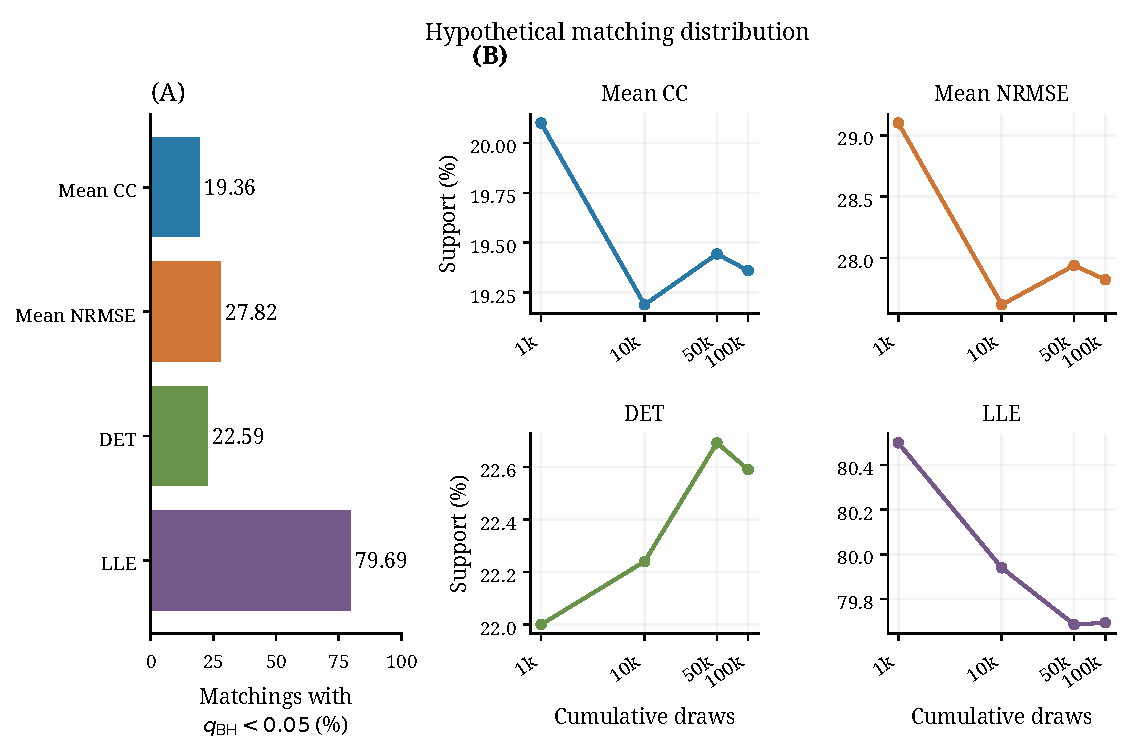
\includegraphics[width=\linewidth,height=.75\textheight,keepaspectratio]{figures/figure_S09.pdf}
\caption{Hypothetical repeated-session dependence. (A) Fractions of 100,000 matchings with $q_{\mathrm{BH}}<0.05$ for the four headline metrics, applying BH7 within matching. All four median directions were preserved in every sampled matching. (B) Cumulative support frequencies at 1k/10k/50k/100k draws. These are summaries of a hypothetical matching distribution, not probabilities of true significance or participant recovery.}\label{fig:supp_repeated}
\end{figure}
\end{landscape}
\subsection{Symbolic Dynamics}\label{sec:supp_14}
Exploratory symbolic analysis encoded PPG-derived peak-to-peak intervals (PPI) at 60/120/180 s. Peaks were detected without extra smoothing, using minimum separation $\lceil0.30f_s\rceil$ samples and prominence 0.20 times the 95th--5th percentile amplitude range. PPI was the successive peak-index difference divided by $f_s$. Acceptance required finite PPI, no intervals outside 0.30--2.00 s, peak-span coverage $\geq90\%$, and at least $\max\{3,\lceil T/2\rceil-2\}$ intervals for duration $T$ seconds. Relative changes above 0.20 were diagnostic, not rejection criteria.

Within each accepted window, PPI was quantized into six equal-width levels between minimum and maximum. Internal-edge values entered the upper bin; constant sequences used level zero. Overlapping three-symbol words were assigned to 0V when both adjacent differences were zero, 1V when exactly one was zero, and 2V when both were nonzero. 2V combined same-sign 2LV and opposite-sign 2UV changes. Occurrence percentages summed to 100\% within windows, although separately aggregated session-state medians need not. Paired comparisons followed session-state medians of accepted windows.

Table~\ref{tab:supp_symbolic} retains all nine category--duration results, with BH3 within duration. Median 0V effects were positive and 2V effects negative at every duration; 1V was near zero and changed aggregate sign at 180 s. None passed its BH family. The 60-s 0V and 180-s 2V CIs excluded zero; the latter raw p was 0.048441 but q was 0.145323. These CI/raw-test features do not override the exploratory multiplicity result.

Paired effects kept the same sign across all three durations in 17/20 sessions for 0V, 11/20 for 1V, and 14/20 for 2V. Counts include consistently positive or negative sessions, regardless of the aggregate direction, and do not imply equal magnitude. Symbolic proportions provide directional context (Fig.~\ref{fig:supp_symbolic}) outside the primary four-metric claim; they are not direct sympathetic/vagal measures or validated ECG-derived autonomic measures.

\begin{landscape}
\begingroup\small
\setlength{\tabcolsep}{3pt}
\renewcommand{\arraystretch}{1.18}
\stepcounter{supptablepanel}
\begin{longtable}{L{\dimexpr0.08929\linewidth-1.60714\tabcolsep\relax}L{\dimexpr0.08036\linewidth-1.44643\tabcolsep\relax}L{\dimexpr0.08036\linewidth-1.44643\tabcolsep\relax}L{\dimexpr0.10714\linewidth-1.92857\tabcolsep\relax}L{\dimexpr0.17857\linewidth-3.21429\tabcolsep\relax}L{\dimexpr0.11607\linewidth-2.08929\tabcolsep\relax}L{\dimexpr0.11607\linewidth-2.08929\tabcolsep\relax}L{\dimexpr0.10714\linewidth-1.92857\tabcolsep\relax}L{\dimexpr0.12500\linewidth-2.25000\tabcolsep\relax}}
\caption{Exploratory symbolic supporting results.}\label{tab:supp_symbolic}\\
\toprule
Category & Duration (s) & Paired n & $\Delta$ (pp) & 95\% CI (pp) & Raw $p$ & $q_{\mathrm{BH}}$ & $r_{\mathrm{rb}}$ & Direction count\\
\midrule\endfirsthead
\multicolumn{9}{l}{Table~\ref{tab:supp_symbolic} (continued)}\\
\toprule
Category & Duration (s) & Paired n & $\Delta$ (pp) & 95\% CI (pp) & Raw $p$ & $q_{\mathrm{BH}}$ & $r_{\mathrm{rb}}$ & Direction count\\
\midrule\endhead
\bottomrule\endfoot
\bottomrule\endlastfoot
0V & 60 & 20 & +4.04 & [+0.35, +7.18] & 0.053169 & 0.113777 & +0.495 & 14/\allowbreak 20\\
1V & 60 & 20 & +0.41 & [-1.47, +2.23] & 0.498009 & 0.498009 & +0.181 & 10/\allowbreak 20\\
2V & 60 & 20 & -0.91 & [-6.40, +0.37] & 0.075851 & 0.113777 & -0.457 & 13/\allowbreak 20\\
0V & 120 & 20 & +2.32 & [-2.64, +5.63] & 0.474905 & 0.712358 & +0.190 & 13/\allowbreak 20\\
1V & 120 & 20 & +0.03 & [-1.67, +2.13] & 0.927279 & 0.927279 & +0.029 & 10/\allowbreak 20\\
2V & 120 & 20 & -2.30 & [-4.68, +1.78] & 0.329983 & 0.712358 & -0.257 & 12/\allowbreak 20\\
0V & 180 & 20 & +4.58 & [-1.12, +13.94] & 0.164957 & 0.247436 & +0.362 & 13/\allowbreak 20\\
1V & 180 & 20 & -0.06 & [-4.31, +1.95] & 0.956329 & 0.956329 & -0.019 & 10/\allowbreak 20\\
2V & 180 & 20 & -2.67 & [-5.37, -0.44] & 0.048441 & 0.145323 & -0.505 & 15/\allowbreak 20\\
\end{longtable}
\endgroup
{\small All nine tests are exploratory, with BH3 separately within duration. pp denotes percentage points. Direction counts are positive for 0V/1V and negative for 2V; 1V uses a positive reporting convention even at its slightly negative 180-s median.}\par
{\small Same-sign-across-duration counts are 17/20 (0V), 11/20 (1V), 14/20 (2V), including consistently opposite-direction sessions. Effects/CIs use two decimals, raw p/q six, and rank-biserial effects three.}\par
\end{landscape}
\begin{figure}[p]
\centering
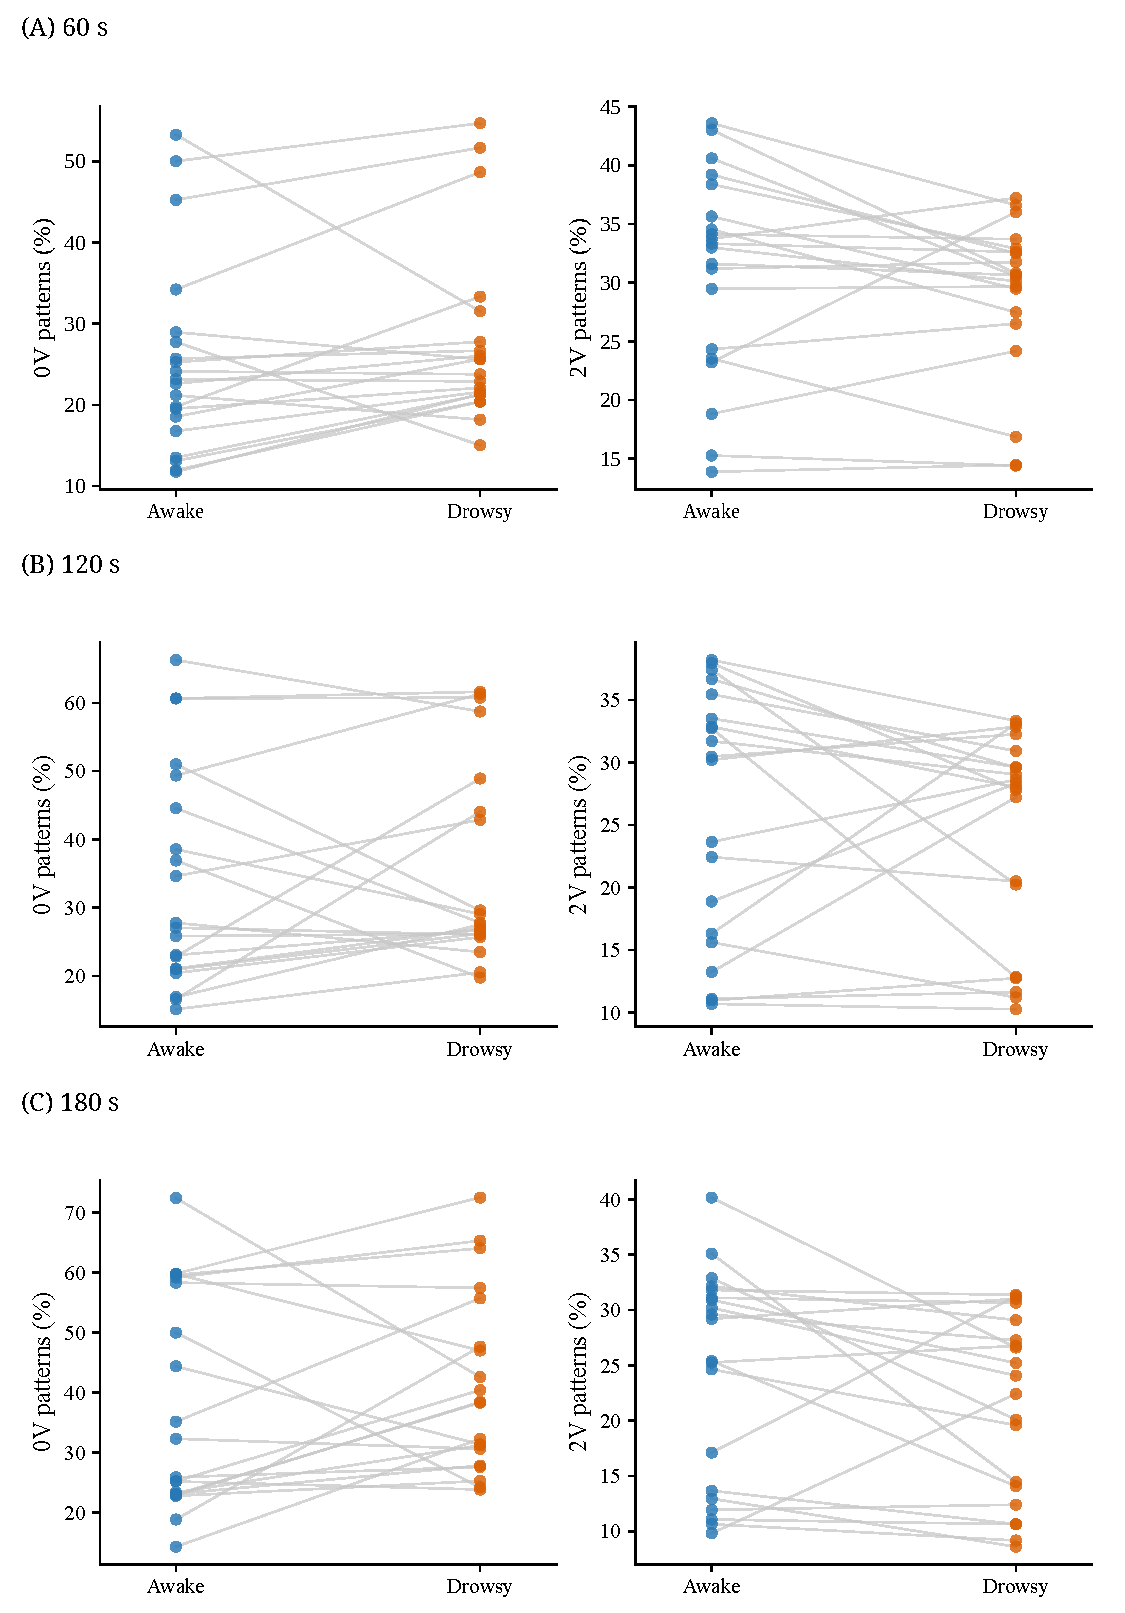
\includegraphics[width=\linewidth,height=.84\textheight,keepaspectratio]{figures/figure_S10.pdf}
\caption{Exploratory symbolic PPI evidence at (A) 60, (B) 120, and (C) 180 s. Existing paired session-state 0V/2V occurrence proportions follow six-level PPI quantization and overlapping three-symbol words. Median 0V changes are positive and 2V changes negative, but none of the nine category--duration tests, including 1V in Table~\ref{tab:supp_symbolic}, passes within-duration BH3. Proportions provide supporting context, not direct sympathetic/vagal activity.}\label{fig:supp_symbolic}
\end{figure}
\subsection{Overall Robustness Summary}\label{sec:supp_15}
Table~\ref{tab:supp_summary} separates nominal effects, direction preservation, uncertainty, and statistical support. Mean CC decreased and Mean NRMSE increased across tested window, label, delay, and dimension settings, with variable magnitudes/CIs and attenuated support under hypothetical grouping.

DET retained its nominal decrease across windows, labels, dimensions, and tested RQA RR/Theiler settings, but became near-zero and positive at non-nominal delays. Embedding-delay dependence is therefore an explicit qualification. LLE retained its decrease across all tested branches and the strongest support in hypothetical grouping, while fit/QC choices changed magnitude and accepted-window counts.

Symbolic evidence remains exploratory. Sensitivities are supportive analyses of the same recordings, rather than independent replications. Unknown participant--session linkage remains unresolved by hypothetical grouping. The matrix assigns no pooled significance, robustness score, or metric ranking.

\begin{landscape}
\begingroup\small
\setlength{\tabcolsep}{3pt}
\renewcommand{\arraystretch}{1.18}
\stepcounter{supptablepanel}
\begin{longtable}{L{\dimexpr0.07194\linewidth-1.15108\tabcolsep\relax}L{\dimexpr0.09353\linewidth-1.49640\tabcolsep\relax}L{\dimexpr0.12950\linewidth-2.07194\tabcolsep\relax}L{\dimexpr0.12950\linewidth-2.07194\tabcolsep\relax}L{\dimexpr0.12230\linewidth-1.95683\tabcolsep\relax}L{\dimexpr0.15108\linewidth-2.41727\tabcolsep\relax}L{\dimexpr0.13669\linewidth-2.18705\tabcolsep\relax}L{\dimexpr0.16547\linewidth-2.64748\tabcolsep\relax}}
\caption{Overall robustness evidence matrix.}\label{tab:supp_summary}\\
\toprule
Metric & Nominal 60-s & Window length & Label rules & $\tau/m$ & Metric-specific estimator settings & Hypothetical grouping & Interpretation limit\\
\midrule\endfirsthead
\multicolumn{8}{l}{Table~\ref{tab:supp_summary} (continued)}\\
\toprule
Metric & Nominal 60-s & Window length & Label rules & $\tau/m$ & Metric-specific estimator settings & Hypothetical grouping & Interpretation limit\\
\midrule\endhead
\bottomrule\endfoot
\bottomrule\endlastfoot
Mean CC & Decrease; BH support & Direction preserved; uncertainty varies & Direction preserved; T60 CI spans zero & Direction preserved; some CIs span zero & Not tested separately here & Direction preserved; support attenuated & Magnitude/\allowbreak support depend on setting; session-level forecastability\\
Mean NRMSE & Increase; BH support & Direction preserved; magnitude varies & Direction preserved; magnitudes differ & Direction preserved; some CIs span zero & Not tested separately here & Direction preserved; support attenuated & Magnitude/\allowbreak support depend on setting; session-level forecastability\\
DET & Decrease; BH support & Direction preserved; 30/\allowbreak 180-s CIs span zero & Direction preserved; magnitudes differ & Delay-sensitive; dimension direction preserved & RR/\allowbreak Theiler direction preserved; RR=0.01 support weaker & Direction preserved; support attenuated & Delay-dependent recurrence-line organization; not physical determinism\\
LLE & Decrease; BH support & Direction preserved; uncertainty varies & Direction preserved; T30 CI spans zero & Direction preserved; magnitude varies & Direction preserved; fit/\allowbreak QC retention and magnitude vary & Direction preserved; strongest support retained in this analysis & Finite-window divergence; QC changes cohort; no participant inference\\
Symbolic & Exploratory; no BH support & 0V/\allowbreak 2V directional context at 60/\allowbreak 120/\allowbreak 180 s & Not tested & Not tested & Not tested & Not tested & Outside primary claim; no direct autonomic interpretation\\
\end{longtable}
\endgroup
{\small Descriptors distinguish median direction, CI uncertainty, and correction-specific support within tested configurations. Untested cells do not imply stability. Symbolic results are outside the primary four-metric claim, and unknown participant linkage remains a limitation.}\par
\end{landscape}
\end{document}
